\chapter{Corrections and Unfolding Procedure}\label{section:star_corrections}
After subtraction of accidental and non-SD backgrounds, the data was corrected for detector inefficiencies to obtain the inclusive distributions of charged particles and particle to antiparticle (pion, kaon, proton and their antiparticle) multiplicity ratios. These corrections include:
\begin{itemize}
	\item event-by-event weights due to vertex reconstruction efficiency:
\begin{equation}
w_\textrm{ev}^\textrm{vrt}\left(n_\textrm{vrt}^\textrm{global}, |\Delta z_0|\right)=\frac{1}{\epsilon_\textrm{vrt}\left(n_\textrm{vrt}^\textrm{global}, |\Delta z_0|\right)}\cdot\frac{1}{\epsilon_\textrm{vrt}^\textrm{veto}\left(n_\textrm{vrt}^\textrm{global}, |\Delta z_0|\right)}
\label{eq:vertexCorrection}
\end{equation}
where the 	$|\Delta z_0|$ dependence is only applicable for events with $n_\textrm{vrt}^\textrm{global}$ as described in Sec.~\ref{section:star_vertex}.
	\item track-by-track weights due to track reconstruction efficiency, track backgrounds from non-primary tracks, migrations of tracks into and out of the fiducial region:
\begin{equation}
w_\textrm{trk}\left(p_\textrm{T},\eta,V_{z}\right)=\frac{1-f_\textrm{bkg}\left(p_\textrm{T},\eta\right)-f_\textrm{fake}\left(p_\textrm{T},\eta\right)}{\epsilon_\textrm{TPC}\left(p_\textrm{T},\eta,V_{z}\right)\epsilon_\textrm{TOF}\left(p_\textrm{T},\eta,V_{z}\right)}f_\textrm{okr}\left(p_\textrm{T},\eta\right)
\label{eq:trackCorrection}
\end{equation}
where: $\epsilon_\textrm{TPC}\left(p_\textrm{T},\eta,V_{z}\right)$ is TPC track reconstruction efficiency~\cite{supplementaryNote}, $\epsilon_\textrm{TOF}\left(p_\textrm{T},\eta,V_{z}\right)$ is TOF matching efficiency~\cite{supplementaryNote}, $f_\textrm{okr}\left(p_\textrm{T},\eta\right)$ is a~factor accounting for migrations of tracks into and out of the~fiducial region, $f_\textrm{bkg}\left(p_\textrm{T},\eta\right)$ is a~fraction of background tracks, and $f_\textrm{fake}\left(p_\textrm{T},\eta\right)$ is a~fraction of fake tracks.
\item event-by-event (for $n_\textrm{ch}$ distribution ) or track-by-track (for $p_\textrm{T}$, $\bar{\eta}$ distributions) weights, $f_{\xi}$, due to migrations of events between three $\xi$ regions.
\end{itemize}
Additionally, the obtained distributions were corrected for BBC-small efficiency, $\epsilon_\textrm{BBC}$, using the following weight:
\begin{equation}
w_\textrm{BBC} = \frac{1}{\epsilon_\textrm{BBC}}
\label{eq:bbcCorrection}
\end{equation} 

In the following sections, the correction procedure   for each of the measured distributions is presented separately.
The uncorrected distributions in a wider range  are shown in \cref{fig:nonSDnsel,fig:nonSDpt,fig:nonSDera}.

%multiplicity
\section[Correction to $dN/dn_\textrm{sel}$]{Correction to $\mathbf{dN/dn_\textrm{sel}}$}\label{section:star_dNdnch}
In order to express the multiplicity distribution in terms of the number of charged particles, $n_\textrm{ch}$, instead of the number of selected tracks, $n_\textrm{sel}$.%,  the observed $n_\textrm{sel}$ distribution was corrected for detector effects after subtraction of accidental and non-SD backgrounds. 
The  following procedure based on the Bayesian unfolding~\cite{unfolding:2016mok,unfolding:DAgostini} was used. First, the~$n_\textrm{sel}$ distribution was corrected for vertex reconstruction effects by applying event-by-event weights, $w_\textrm{ev}^\textrm{vrt}(n_\textrm{vrt}^\textrm{global},|\Delta z_0|)$. The number of events in which $n_\textrm{ch}$ are produced, $N_\textrm{ev}(n_\textrm{ch})$, can be associated with the number of events in which $n_\textrm{sel}$ are reconstructed, $N_\textrm{ev}(n_\textrm{sel})$.
\begin{comment}
\begin{equation}
N_\textrm{ev}\left(n_\textrm{ch}|n_\textrm{sel}\right)=N_\textrm{ev}\left(n_\textrm{sel}\right)\cdot P\left(n_\textrm{ch}|n_\textrm{sel}\right)
\end{equation}
where $P(n_\textrm{ch}|n_\textrm{sel})$ is the conditional probability of having $n_\textrm{ch}$ charged particles in an event in which  $n_\textrm{sel}$ tracks were found.
\end{comment}
Since there are several possible $n_\textrm{sel}$ observed in  $n_\textrm{ch}$ event,  $N_\textrm{ev}(n_\textrm{ch})$ is given by:
\begin{equation}
\begin{array}{ccccc}
N_\textrm{ev}(n_\textrm{ch})&=&&\displaystyle\sum_{n_\textrm{sel}=0}P(n_\textrm{ch}|n_\textrm{sel})\cdot N_\textrm{ev}(n_\textrm{sel})\\
&=&\frac{1}{\epsilon_{m}(n_\textrm{ch})\epsilon_{r}(n_\textrm{ch})}&\displaystyle\sum_{n_\textrm{sel}=2}^{8}P(n_\textrm{ch}|n_\textrm{sel})\cdot N_\textrm{ev}(n_\textrm{sel})
\end{array}
\end{equation}
where:
\begin{description}
	\item $P(n_\textrm{ch}|n_\textrm{sel})$ is the conditional probability of having $n_\textrm{ch}$ charged particles in an event in which  $n_\textrm{sel}$ tracks were found,
	\item $\epsilon_{m}(n_\textrm{ch})$ is a factor, which recovers events that are lost due to TPC track reconstuction and  TOF matching inefficiencies, i.e. those with $n_\textrm{ch}\geq2$ but $n_\textrm{sel}<2$,
	\item $\epsilon_{r}(n_\textrm{ch})$ is a factor, which recovers  events which are lost due to fake tracks, i.e. those with $n_\textrm{ch}\leq 8$ but $n_\textrm{sel}> 8$. It was checked that this effect is negligible (smaller than $1\permil$) and can be omitted. 
\end{description}
Figure~\ref{fig:correctionSTAR} shows $\epsilon_{m}(n_\textrm{ch})$  in three ranges of $\xi$. It was derived from MC and varies from about $25\%$ for $n_\textrm{ch}=2$ to $95\%$ for $n_\textrm{ch}=8$. Since there are additional data-driven corrections to \ac{TPC} and TOF efficiences,  MC simulations were modified by randomly removing or adding tracks. This was done in accordance with differences in the~efficiencies between data and MC. 
Figure~\ref{fig:correctionSTAR_syst} shows  $\epsilon_{m}(n_\textrm{ch})$ calculated in three ranges of $\xi$ using no-pile-up PYTHIA~8 and EPOS SD+SD$^\prime$. The~differences between
these two models, which are up to $8\%$ for $n_\textrm{ch}=2$ and $0.1<\xi<0.2$, were symmetrized and taken as a~systematic uncertainty.


\begin{figure}[h!]
	\centering
		\begin{subfigure}{.49\textwidth}
			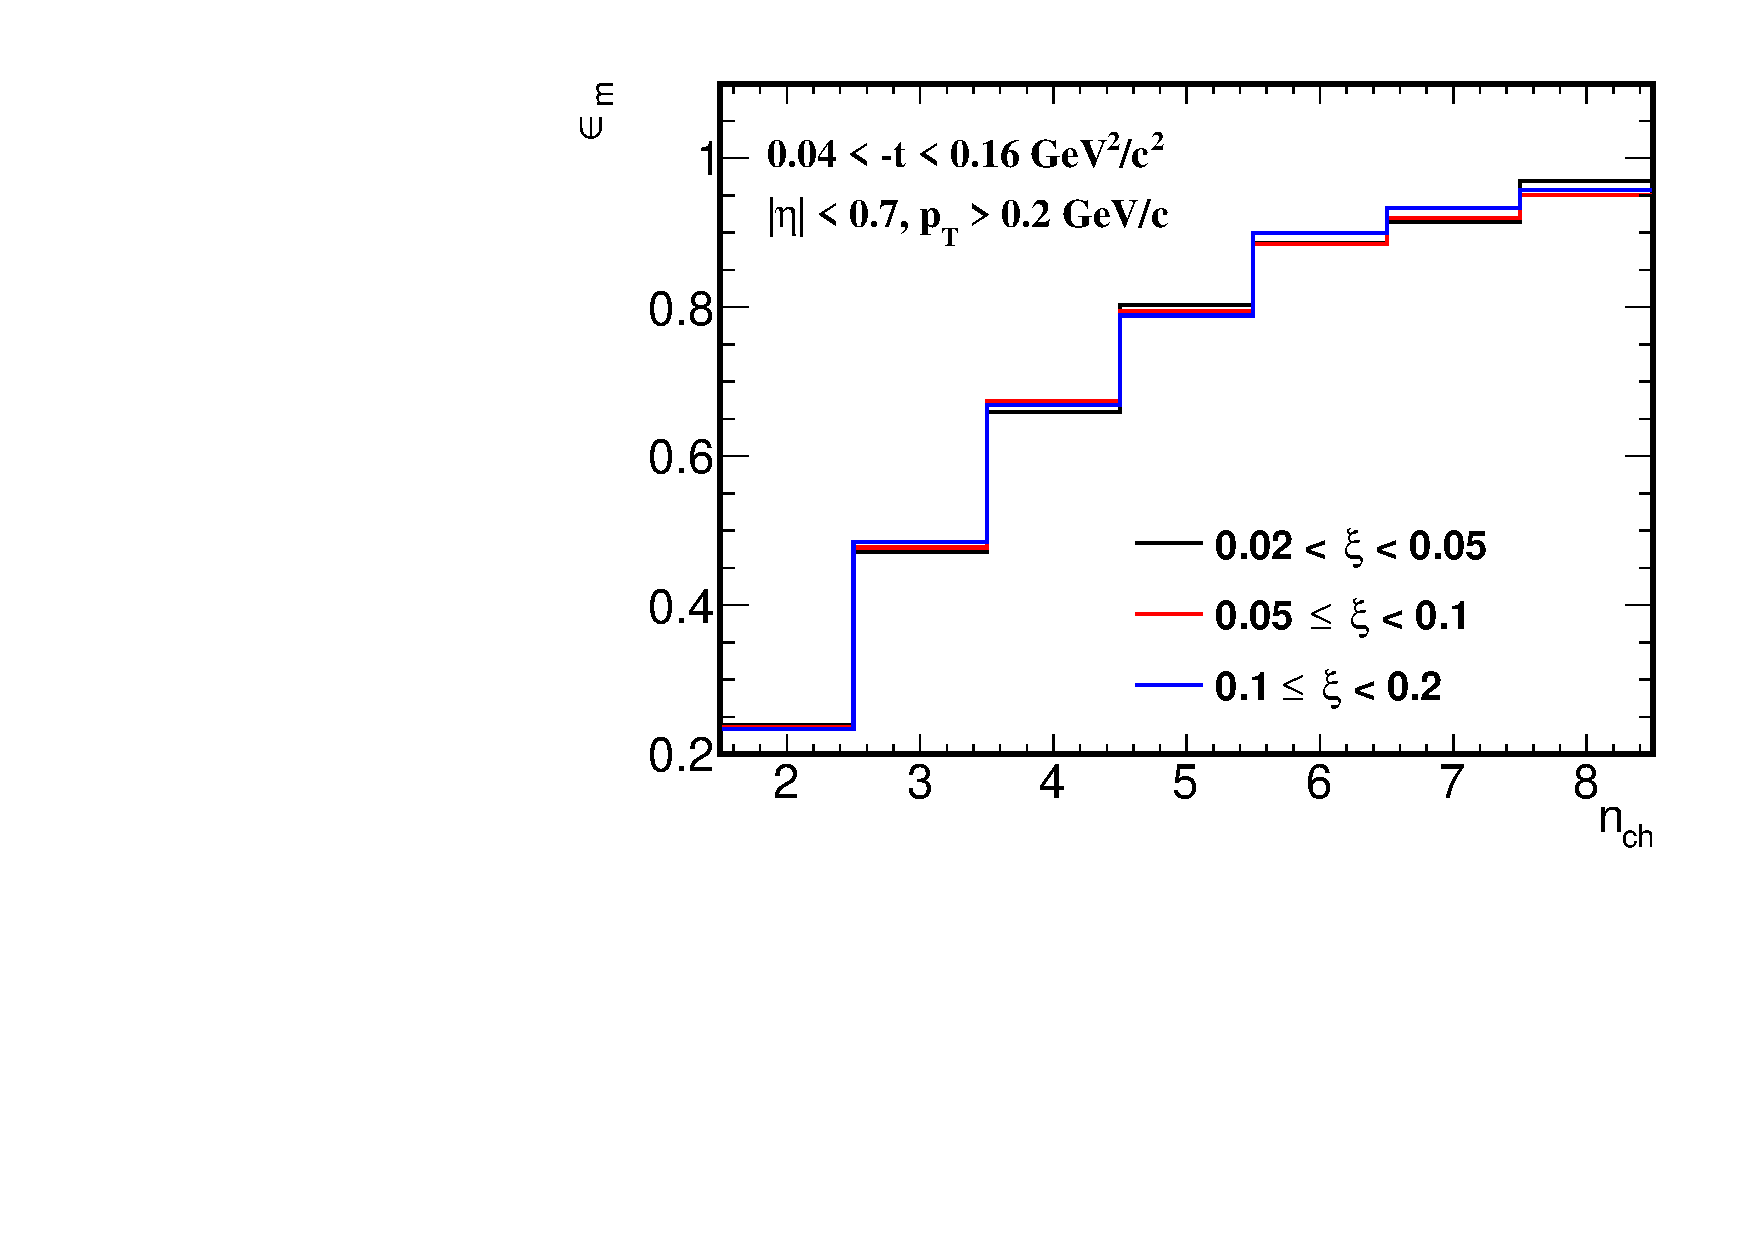
\includegraphics[width=\textwidth,page=1]{chapters/chrgSTAR/img/unfolding/correction_0.pdf}
		\end{subfigure}
		\begin{minipage}{.49\textwidth}
			\caption{$\epsilon_{m}(n_\textrm{ch})$  calculated separately in three ranges of $\xi$ using PYTHIA~8 embedding MC.}
			\label{fig:correctionSTAR}
		\end{minipage}
	
\end{figure}


\begin{figure}[h!]
	\centering
	\begin{subfigure}{.47\textwidth}
		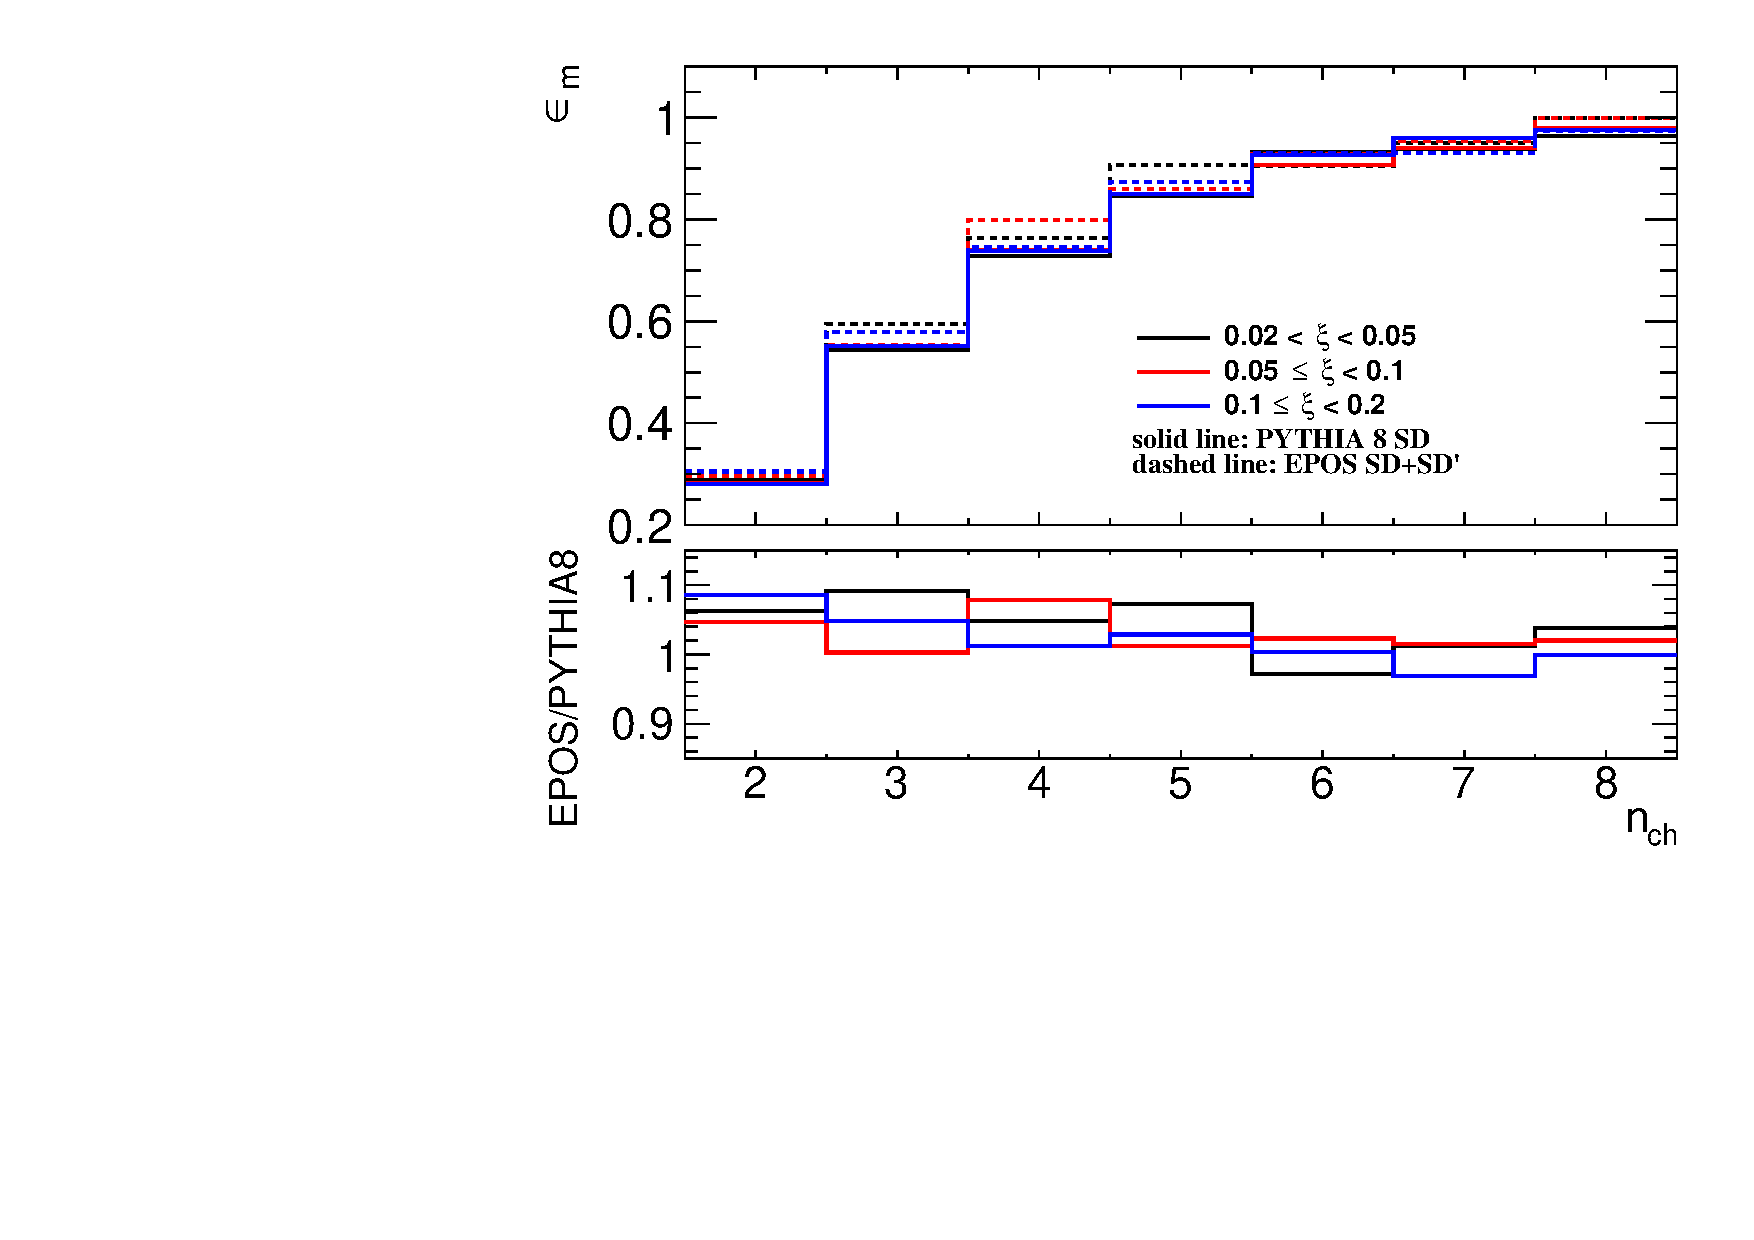
\includegraphics[width=\textwidth,page=1]{chapters/chrgSTAR/img/unfolding/nch_m2_nsel_s2.pdf}
	\end{subfigure}
	\begin{minipage}{.48\textwidth}
		\caption{Comparison of $\epsilon_{m}(n_\textrm{ch})$  calculated separately in three ranges of $\xi$ using PYTHIA~8 SD and EPOS SD+SD$^\prime$ no-pile-up MCs.}
		\label{fig:correctionSTAR_syst}
	\end{minipage}
	
\end{figure}

\noindent The  probability $P(n_\textrm{ch}|n_\textrm{sel})$ can be derived using Bayes' theorem, which can be stated mathematically in terms of charged particle and charged track multiplicities as:
\begin{equation}
P\left(n_\textrm{ch}\right)\cdot P\left(n_\textrm{sel}|n_\textrm{ch}\right) = P\left(n_\textrm{ch}|n_\textrm{sel}\right)\cdot P\left(n_\textrm{sel}\right)
\end{equation}
where: $P(n_\textrm{sel})$ and $P(n_\textrm{ch})$ are probabilities of observing $n_\textrm{sel}$ and $n_\textrm{ch}$ respectivelly, $P(n_\textrm{ch}|n_\textrm{sel})$ and $P(n_\textrm{sel}|n_\textrm{ch})$ are conditional probabilities.
 
\noindent 
In order to improve the estimate of $P(n_\textrm{ch}|n_\textrm{sel})$, the~unfolding  is done iteratively:
\begin{itemize}
	\item In the~first iteration, it is assumed that: \\
	\begin{eqnarray}
	P(n_\textrm{ch}|n_\textrm{sel}) = P = P^{\textrm{MC}}(n_\textrm{sel}|n_\textrm{ch})\frac{P^\textrm{MC}(n_\textrm{ch})}{P^\textrm{MC}(n_\textrm{sel})}
	\end{eqnarray}
	\begin{equation}
	N_\textrm{ev}(n_\textrm{ch})=\frac{1}{\epsilon_{m}(n_\textrm{ch})}\sum_{n_\textrm{sel}=2}^{8}N_\textrm{ev}(n_\textrm{sel})\cdot P
	\end{equation}
	where $P^{\textrm{MC}}(n_\textrm{sel}|n_\textrm{ch})$, $P^\textrm{MC}(n_\textrm{ch})$ and $P^\textrm{MC}(n_\textrm{sel})$ are obtained from MC. $P^{\textrm{MC}}(n_\textrm{sel}|n_\textrm{ch})$ is the~same for each iteration.
	
	\item In the $(i+1)$th iteration we have:
	\begin{equation}
	P^{i+1}=P^{\textrm{MC}}(n_\textrm{sel}|n_\textrm{ch})\frac{N_\textrm{ev}^{i}(n_\textrm{ch})}{N_\textrm{ev}(n_\textrm{sel})}
	\end{equation}
	\begin{equation}
	N_\textrm{ev}^{i+1}(n_\textrm{ch})=\frac{1}{\epsilon_{m}(n_\textrm{ch})}\sum_{n_\textrm{sel}=2}^{8}N_\textrm{ev}(n_\textrm{sel})\cdot P^{i+1}
	\end{equation}
	where  $N_\textrm{ev}^i(n_\textrm{ch})$ is calculated in the previous iteration, and $N_\textrm{ev}(n_\textrm{sel})$ is taken from data.
\end{itemize}

The  unfolding matrices $P(n_\textrm{ch}|n_\textrm{sel})$  for each $\xi$ region, shown in Fig.~\ref{fig:responseSTAR}, were obtained from PYTHIA~8 embedding MC and used in all iterations of the above procedure. Similarly to $\epsilon_m(n_\textrm{ch})$, the~matrices were modified in order to take into account differences between data and PYTHIA~8. In order to  increase statistical precision of the~unfolding matrices,   all simulated events were used, i.e. also those with additional fake vertices (with $n_\textrm{sel}$ defined as a~number of primary tracks associated with the~best vertex).
The~systematic uncertainty related to limited statistics in PYTHIA~8 was estimated by performing $50$ pseudo-experiments, in which the~unfolding matrices were smeared according to their statistical uncertainties.
It affects mainly large charged-particle multiplicites, where it is about $8-10\%$ (as shown in Fig.~\ref{fig:responseSTAR_uncert}), and is smaller or at the~same level as  other components contributing  to the~total systematic uncertainty.


\begin{figure}[h!]
	%\vspace{-0.5cm}
	\centering
	\begin{subfigure}{.49\textwidth}
		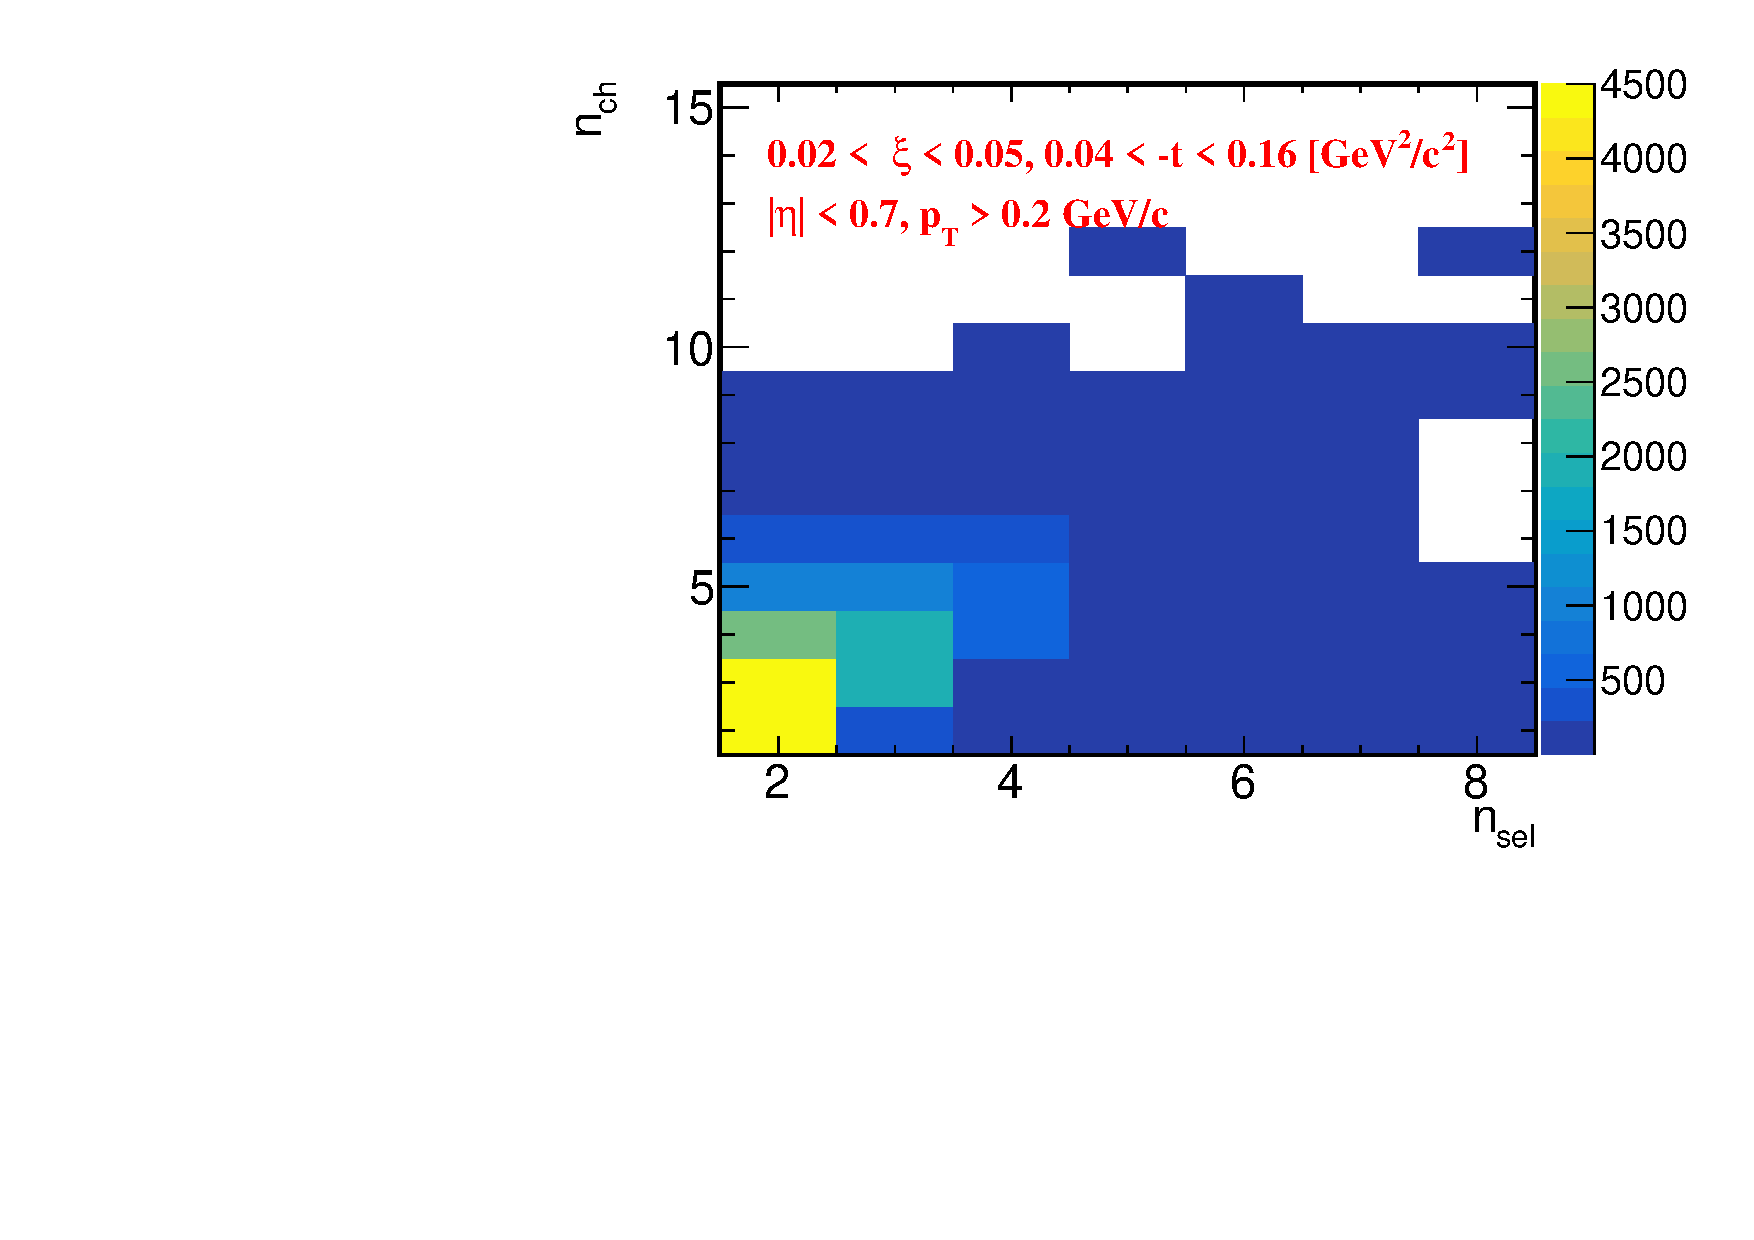
\includegraphics[width=\textwidth,page=1]{chapters/chrgSTAR/img/unfolding/matrix_0.pdf}
	\end{subfigure}
	\begin{subfigure}{.49\textwidth}
		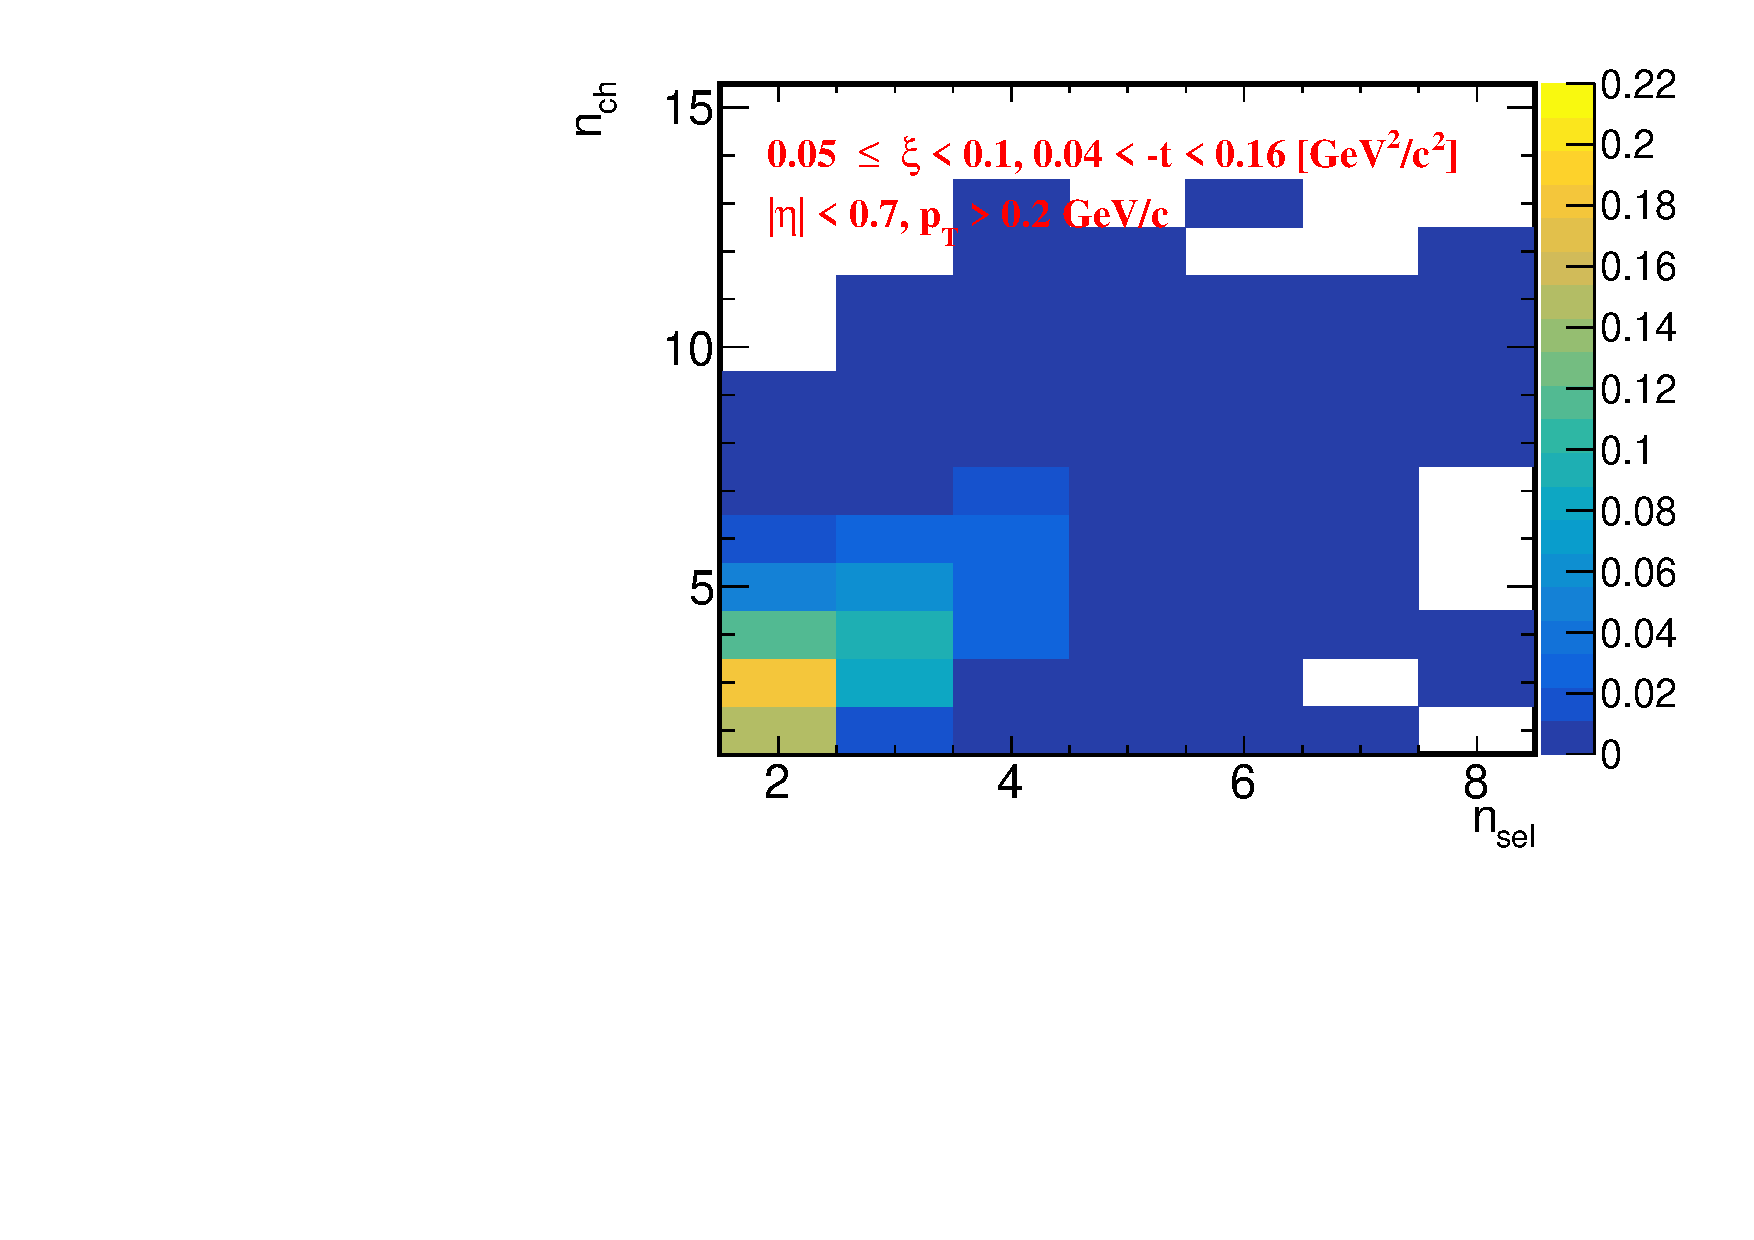
\includegraphics[width=\textwidth,page=1]{chapters/chrgSTAR/img/unfolding/matrix_1.pdf}
	\end{subfigure}
	\begin{subfigure}{.49\textwidth}
		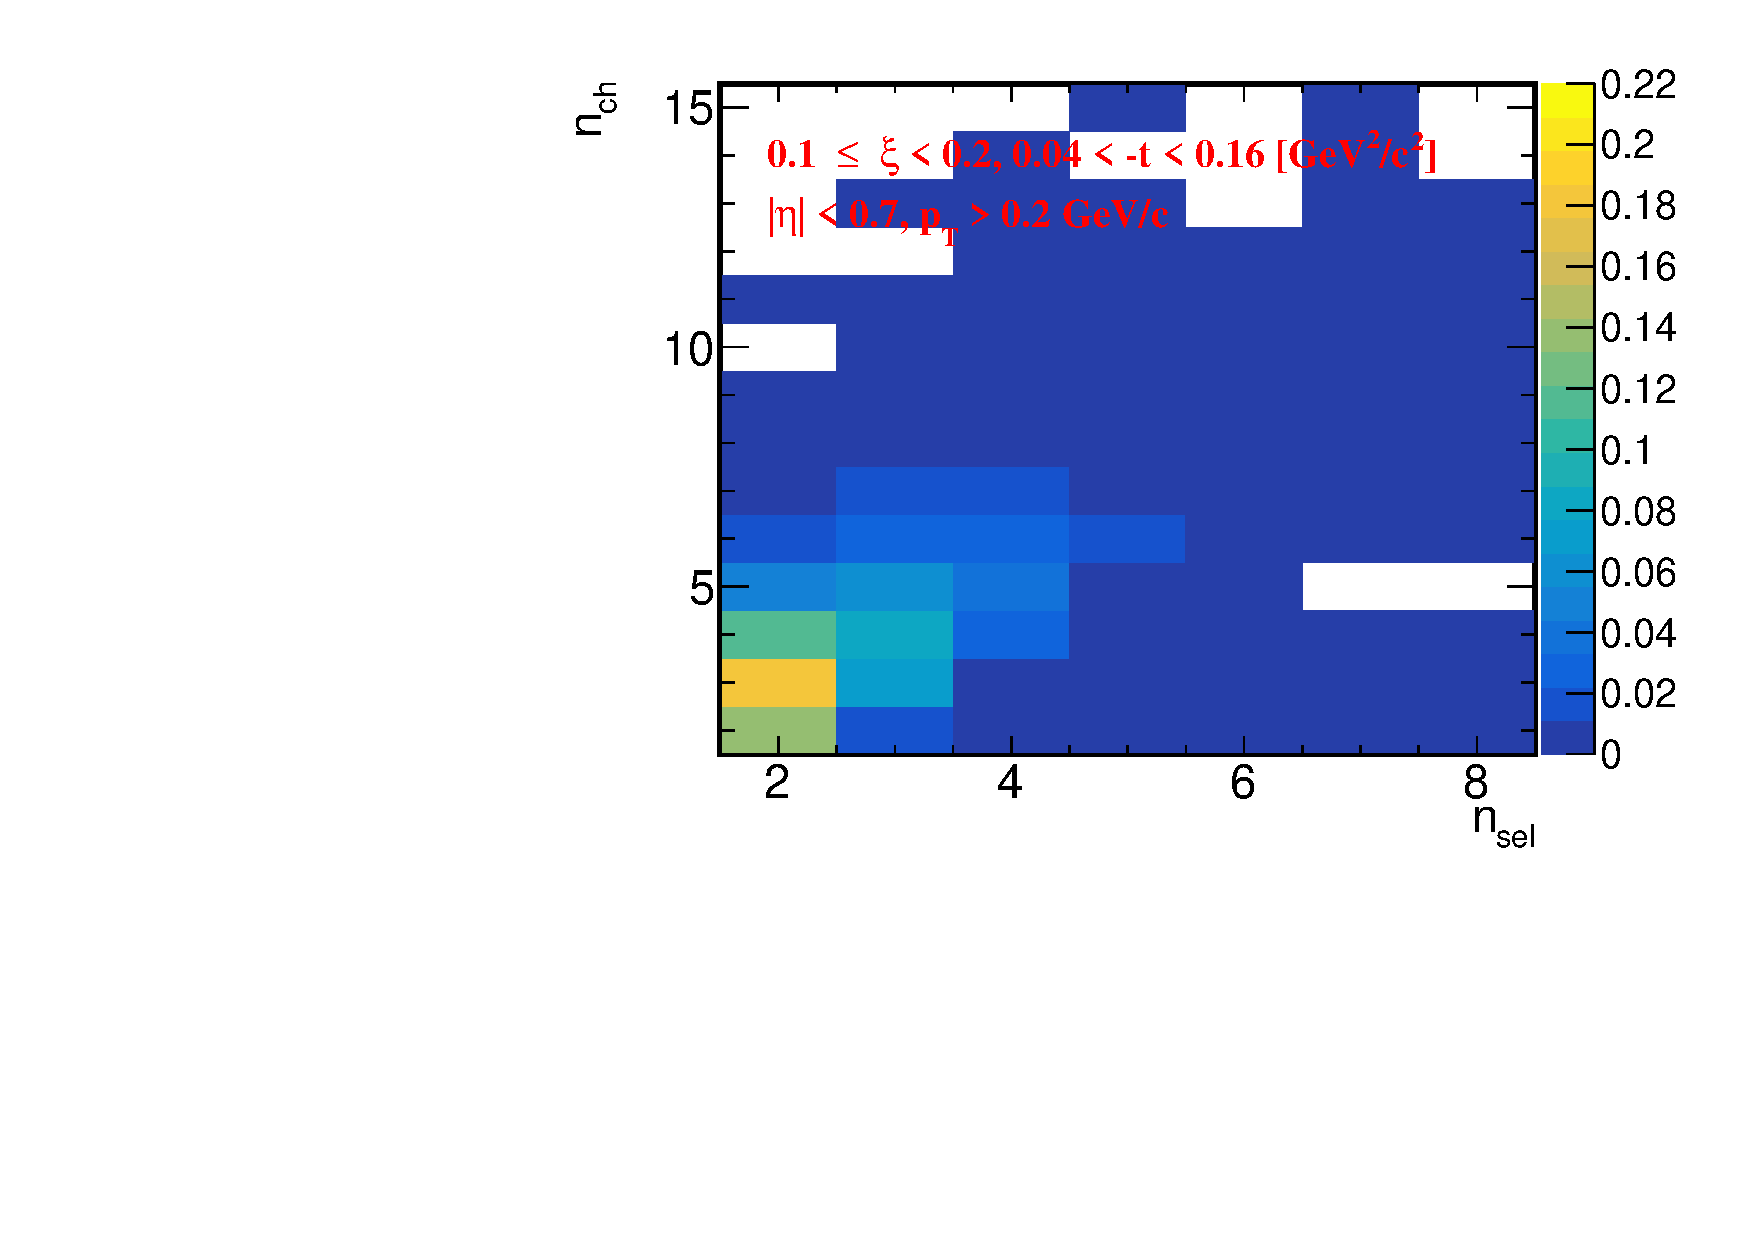
\includegraphics[width=\textwidth,page=1]{chapters/chrgSTAR/img/unfolding/matrix_2.pdf}
	\end{subfigure}
	\begin{minipage}{.49\textwidth}
		\caption{The unfolding matrices calculated  from PYTHIA~8 embedding MC for three ranges of $\xi$ separately.}
		\label{fig:responseSTAR}
	\end{minipage}
	\vspace{-0.5cm}
\end{figure}


\begin{figure}[h!]
	%\vspace{-0.5cm}
	\centering
	\begin{subfigure}{.49\textwidth}
		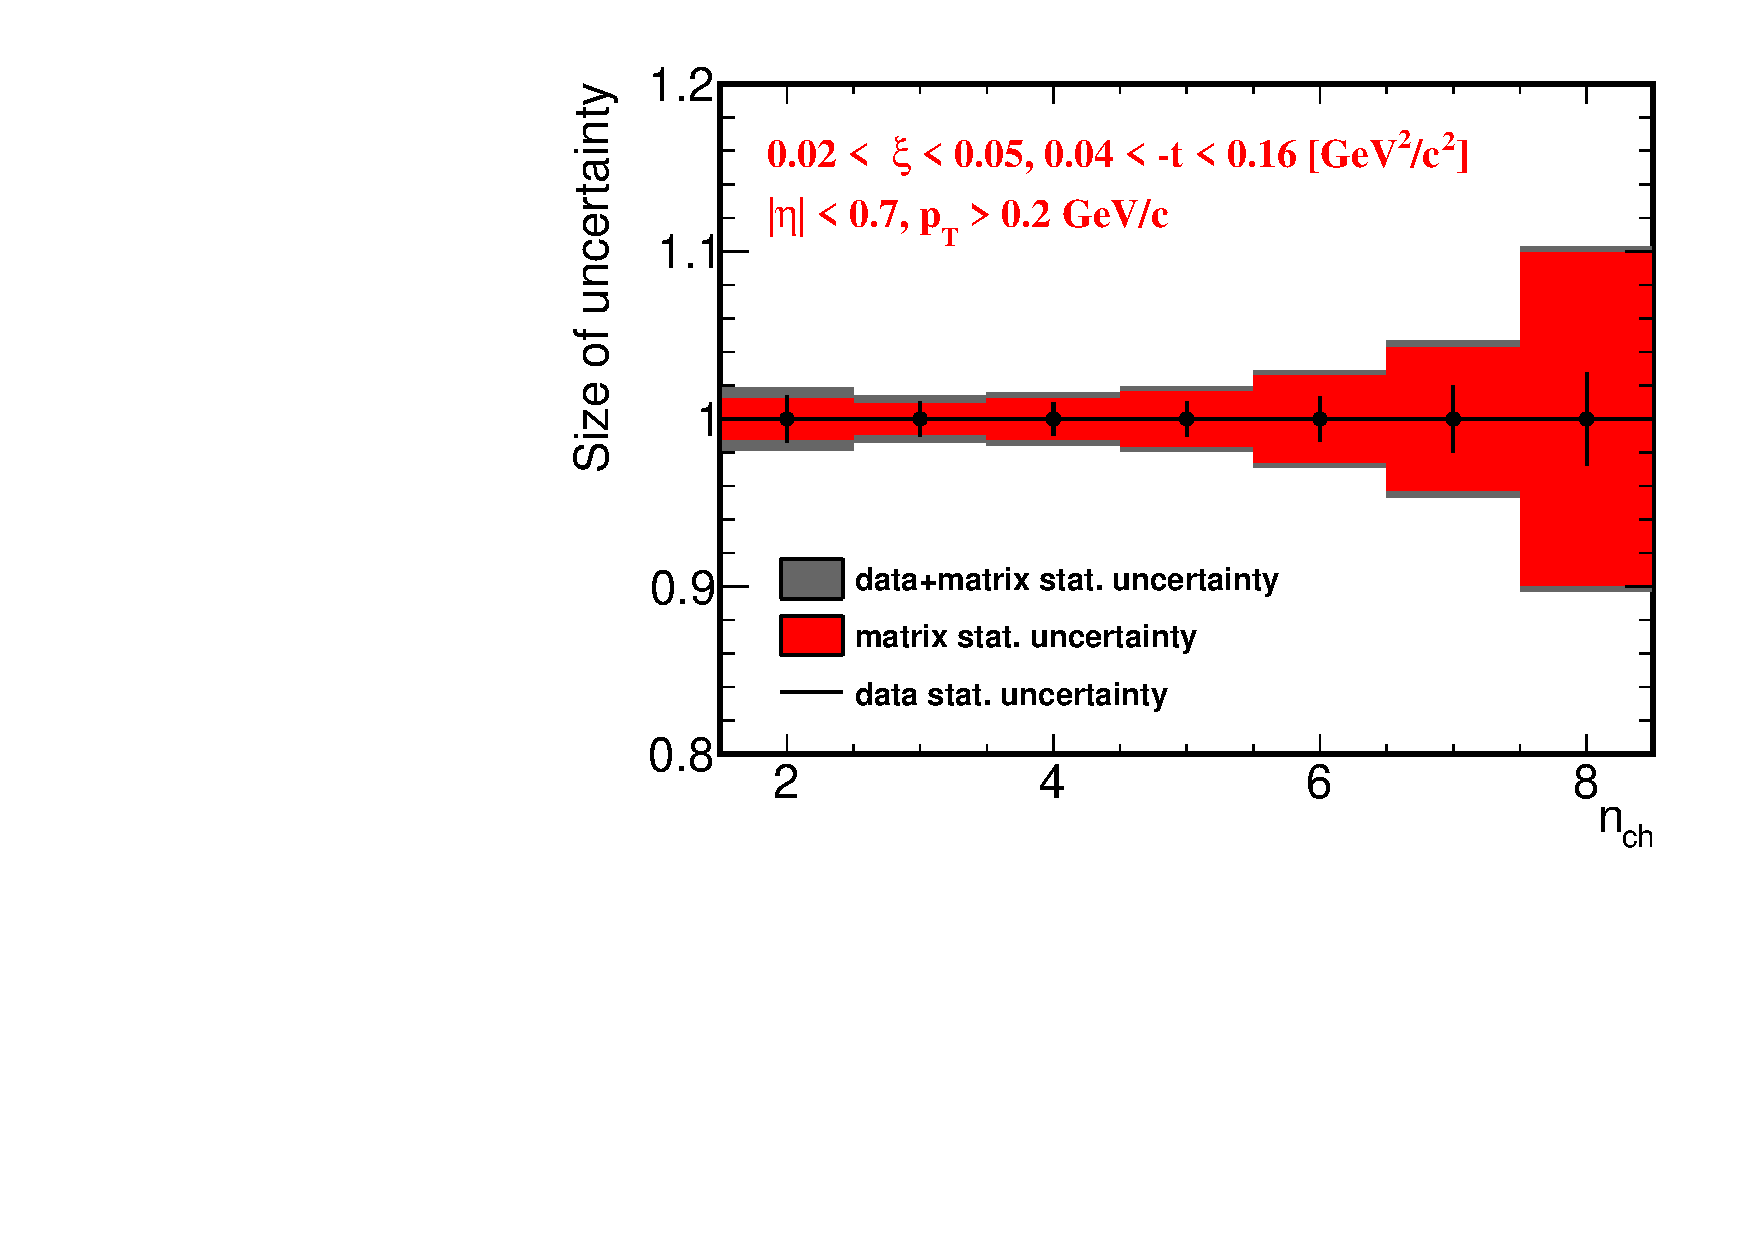
\includegraphics[width=\textwidth,page=1]{chapters/chrgSTAR/img/unfolding/matrix_stat_0.pdf}
	\end{subfigure}
	\begin{subfigure}{.49\textwidth}
		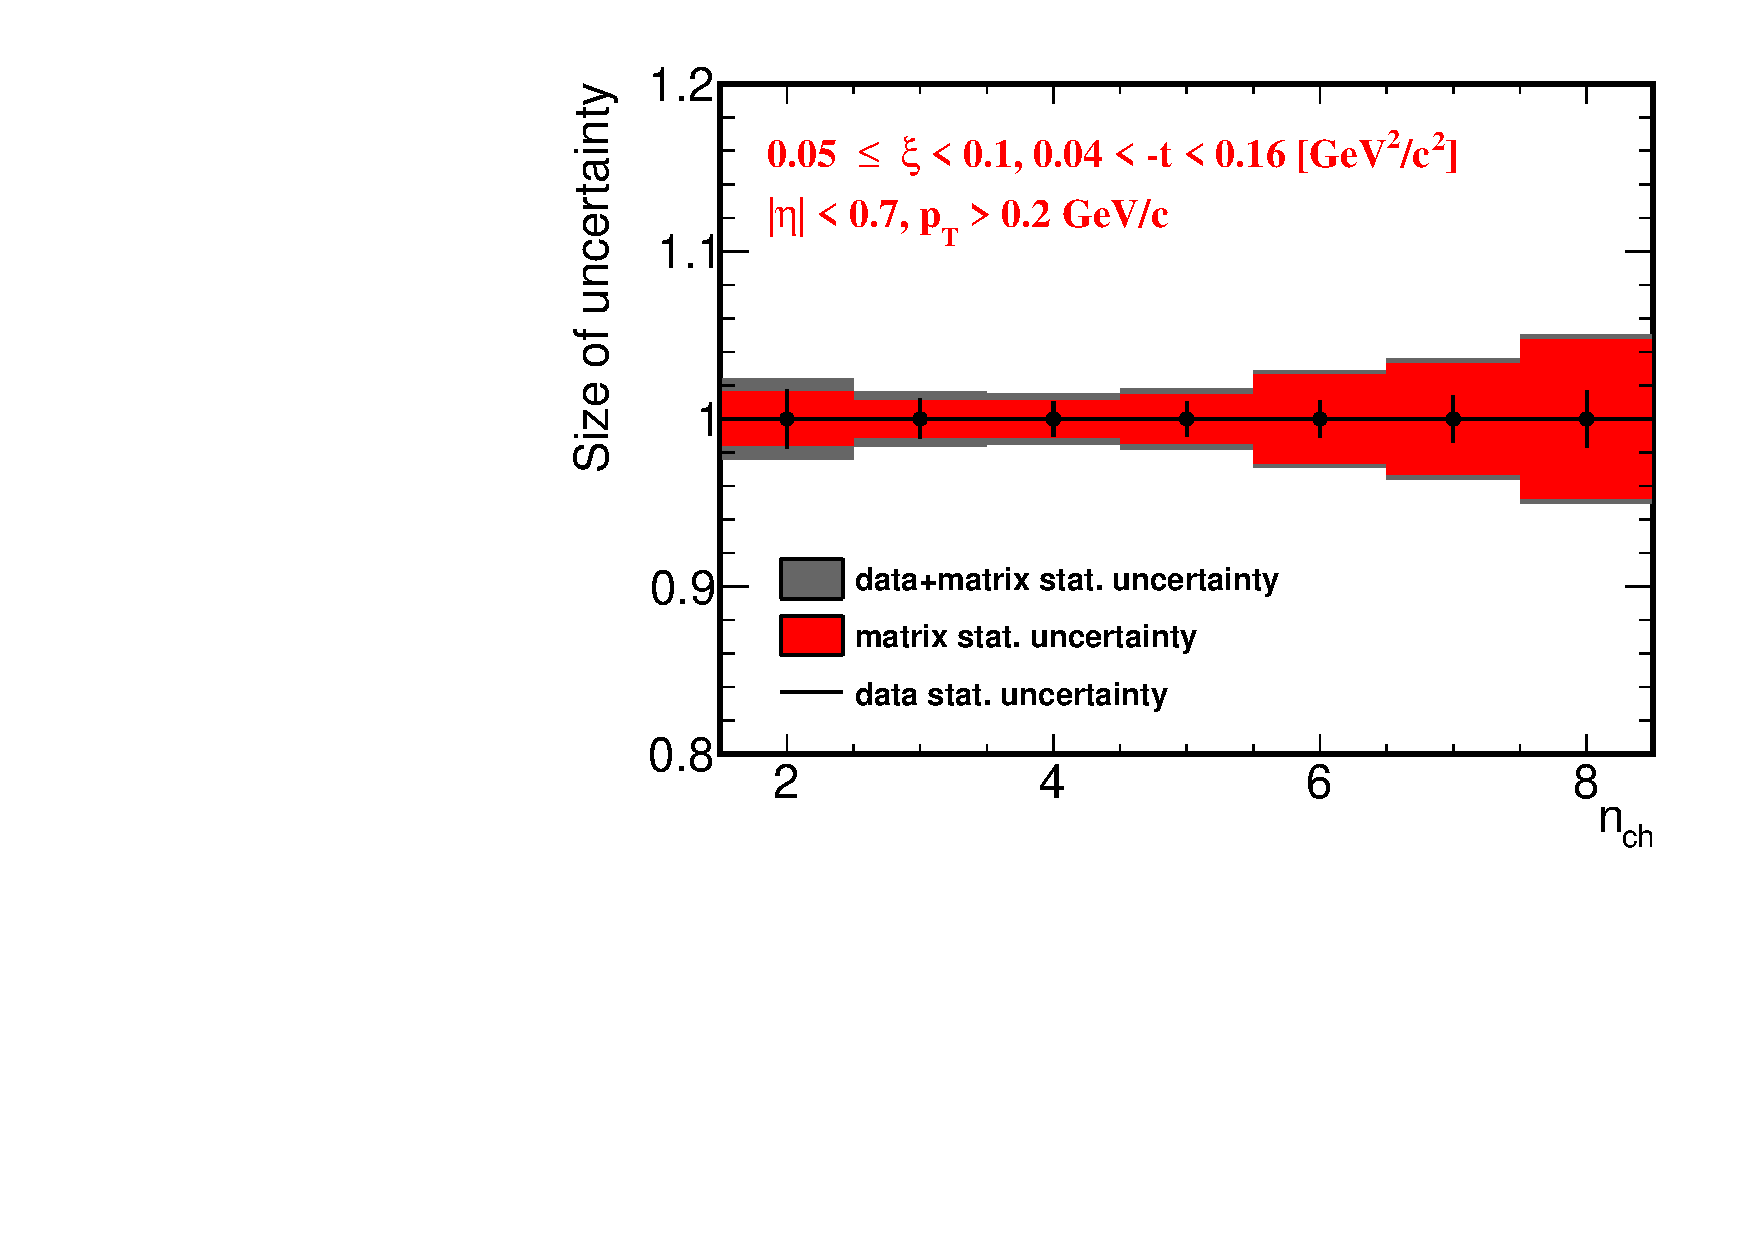
\includegraphics[width=\textwidth,page=1]{chapters/chrgSTAR/img/unfolding/matrix_stat_1.pdf}
	\end{subfigure}
	\begin{subfigure}{.49\textwidth}
		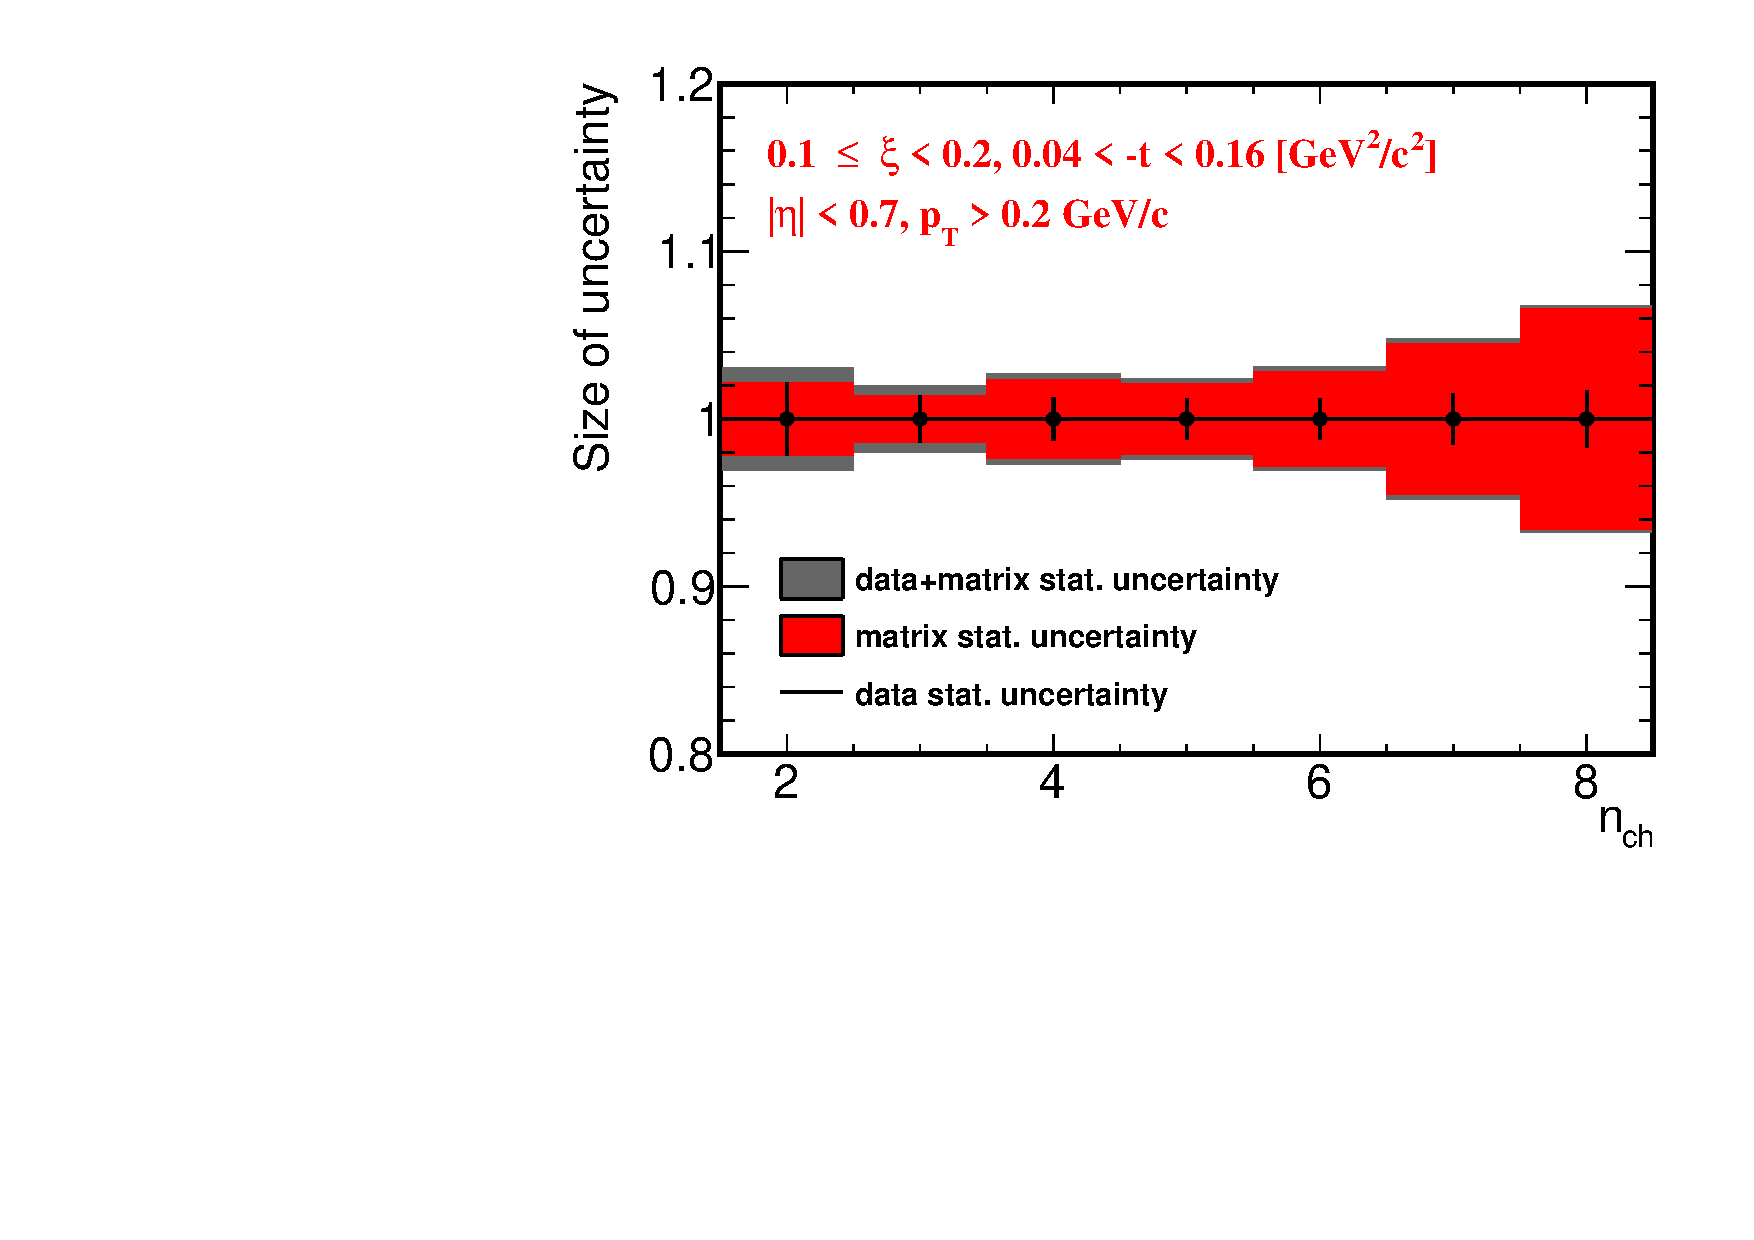
\includegraphics[width=\textwidth,page=1]{chapters/chrgSTAR/img/unfolding/matrix_stat_2.pdf}
	\end{subfigure}
	\begin{minipage}{.49\textwidth}
		\caption{Comparison of  uncertainties  related to data and PYTHIA~8 statistics  for the~charged particle multiplicity in three $\xi$ regions. 
		The~error bars represent uncertainty due to  data
		statistics. The red band shows uncertainty of the~unfolding matrices, while the gray band reflects these two added in quadrature.}
		\label{fig:responseSTAR_uncert}
	\end{minipage}
	%\vspace{-0.5cm}
\end{figure}

The distribution $dN/dn_\textrm{ch}$ obtained after the unfolding procedure
was corrected for BBC-small efficiency, through $w_\textrm{BBC}(n_\textrm{ch})$ weights, and migrations of events between $\xi$ ranges, through $f_{\xi}(n_\textrm{ch})$ weights. Since the unfolding matrices contain track reconstruction efficiencies, non-primary track backgrounds, migrations of tracks into and out of the~fiducial region, the weight $w_\textrm{trk}\left(p_\textrm{T},\eta,V_{z}\right)$ was not used.

\hspace{\parindent} Finally, the $dN/dn_\textrm{ch}$ distribution was normalized to the~total number of events, $N_\textrm{ev}=N$, which was calculated as the integral of the unfolded  distribution.



%\FloatBarrier
%eta, pT
\section{Correction to Transverse Momentum and Pseudorapidity Distributions}\label{section:star_dNdeta_dNdpt}
First the accidental and non-SD backgrounds were subtrated from the $p_\textrm{T}$ and $\bar{\eta}$ distributions. Next, each event was  corrected for vertex reconstruction efficiency by applying $w_\textrm{ev}^\textrm{vrt}(n_\textrm{vrt}^\textrm{global},|\Delta z_0|)$ weights. Then, the tracks were corrected for the track reconstruction efficiency, non-primary track background contribution, track and $\xi$ migrations, BBC-small efficiency (the product of $w_\textrm{trk}(p_\textrm{T},\eta,V_z)$, $f_\xi$ and $w_\textrm{BBC}$ weights was applied, $f_\xi$ and $w_\textrm{BBC}$ were calculated as a~function of true-level $p_\textrm{T}$ and $\bar{\eta}$ separately). 

In order to obtain charged-particle densities, the~$p_\textrm{T}$ and $\bar{\eta}$ distributions   were normalized to unity and scaled by the average charged particle multiplicity in an event $\langle n_\textrm{ch}\rangle$. The latter was calculated from the corrected charged particle multiplicity distribution $dN/dn_\textrm{ch}$ (Sec.~\ref{section:star_dNdnch}).

 The mean particle densities in an event, $\langle p_\textrm{T}\rangle$ and $\langle \bar{\eta}\rangle$, were obtained from the~measured distributions.
%vertexing
\section{Particle Identification}\label{section:star_PIDdEdx}
Specific ionization energy loss, the $dE/dx$, is a function of the~magnitude of a~particle momentum.  In this section the particle identification with help of $dE/dx$  is described.
Due to a~low particle multiplicity and lack of signal in VPDs on the outgoing proton side (presence of the rapidity gap) in SD events, the time of collision is not defined precisely enough, therefore, the particle identification  by the TOF is not possible
and the~analysis was limited to identification only by $dE/dx$. 

The ionization energy loss of charged particles in material
is given by the Bethe-Bloch formula and for
the STAR \ac{TPC} by the more precise Bichsel formula~\cite{Bichsel:2006cs}.
The particle type can be determined by comparison of particle's $dE/dx$ with the Bethe-Bloch (Bichsel) expectations.
Figure \ref{fig:star_dedx} shows the  $dE/dx$ versus rigidity $q\times p$ for particles in $|\eta| < 0.7$. Particles are  well separated at low $|q\times p|$, whereas at higher $|q\times p|$ the $dE/dx$ of different particle species starts to
overlap: $e^\pm$ and $K^\pm$ merge at $\sim0.4$~GeV/c, $K^\pm$ and
$\pi^\pm$ merge at $\sim0.65$~GeV/c, and $p(\bar{p})$ and $\pi^\pm$ merge
at $\sim1$~GeV/c. 
\begin{figure}[b!]
	\centering
	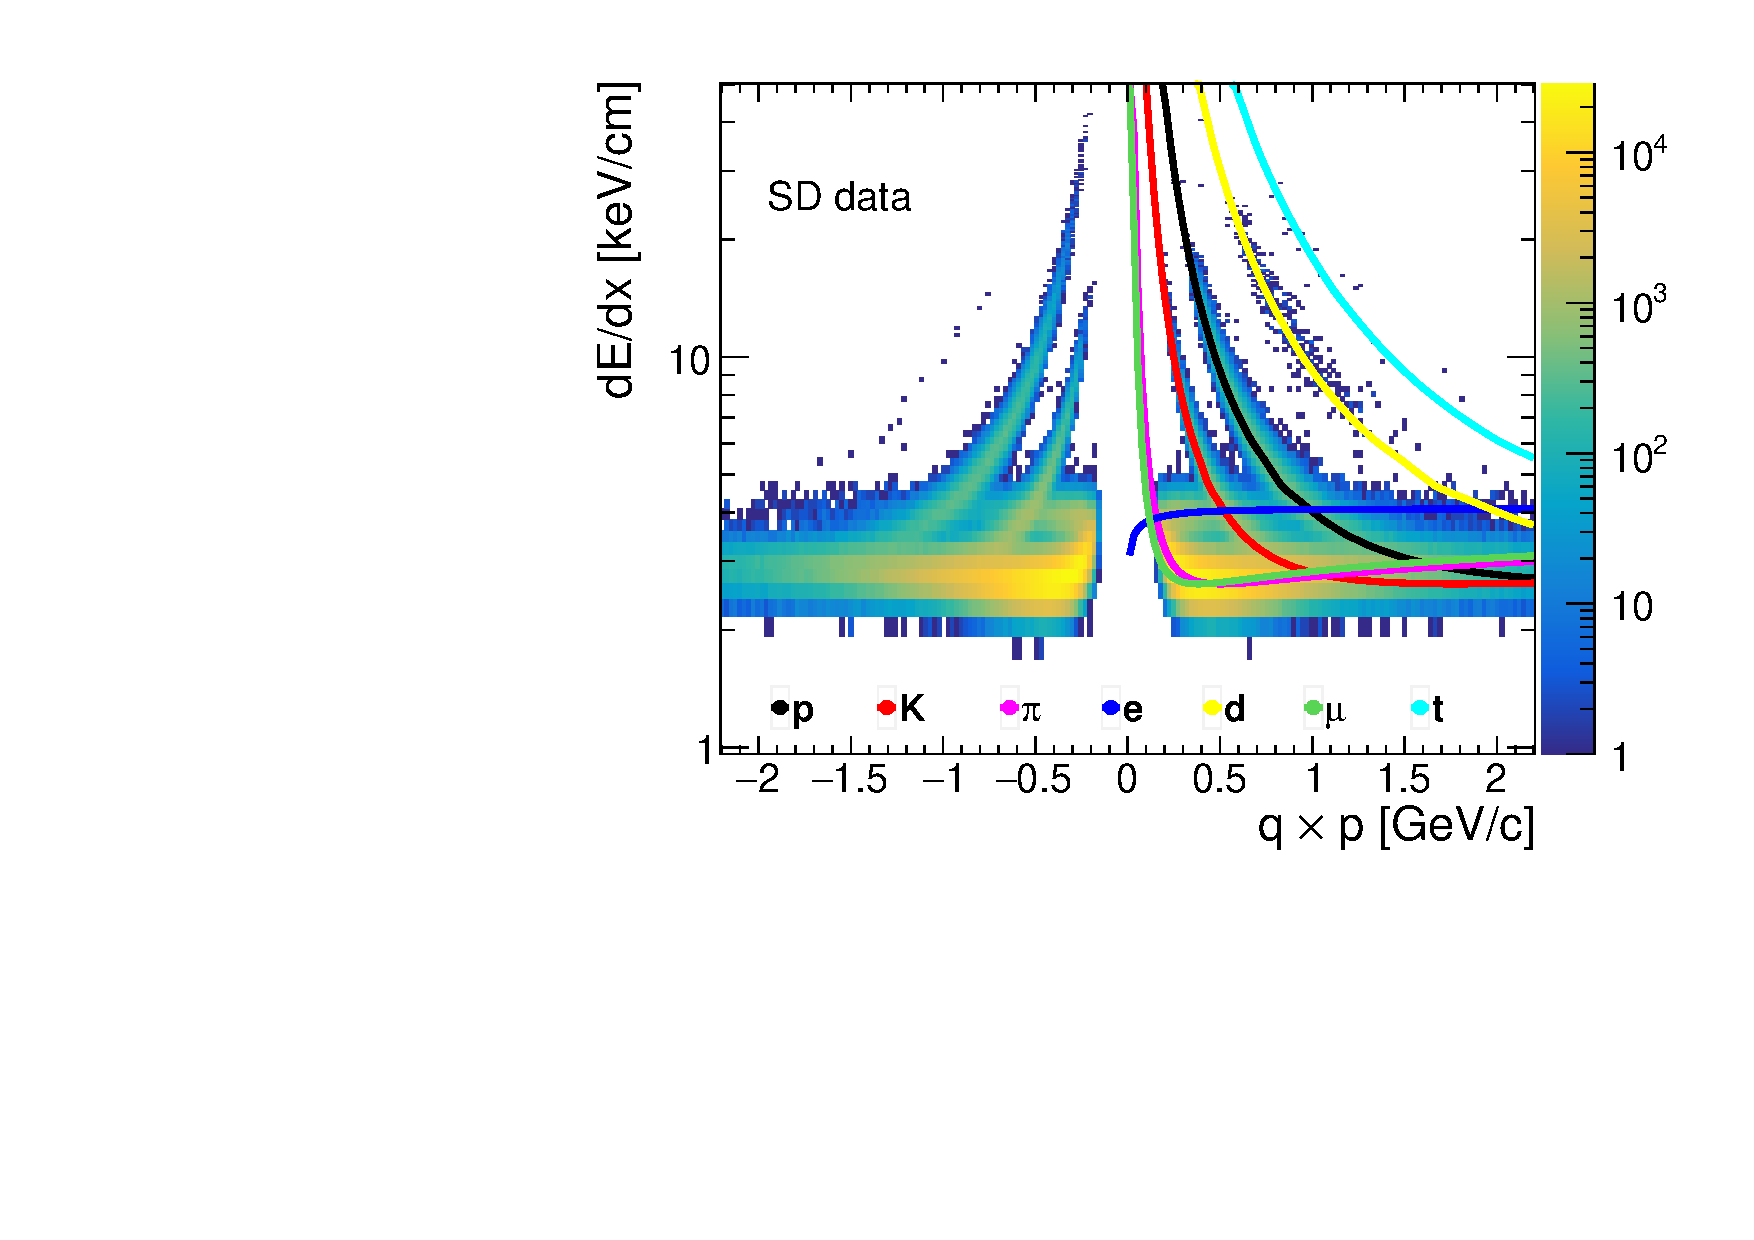
\includegraphics[width=0.65\linewidth, page=1]{chapters/chrgSTAR/img/dEdx/SDT_dEdx.pdf}
	\caption[Specific ionization
	energy loss $dE/dx$ as a function of rigidity $q\times p$ for particles
	in $|\eta| < 0.7$]{Specific ionization
		energy loss $dE/dx$ as a function of rigidity $q\times p$ for particles
		in $|\eta| < 0.7$. The Bichsel predictions for each particle species are also shown.}
	\label{fig:star_dedx}
\end{figure} 
%\FloatBarrier
\noindent Since the $dE/dx$ distribution for a given particle type
is not Gaussian, the following variable for each particle type was defined:
\begin{equation}
n\sigma^i_{dE/dx}=\ln\left(\frac{dE/dx}{(dE/dx)_i^\textrm{{BB}}}\right)/\sigma
\label{eq:nsigma}
\end{equation}
where $(dE/dx)_i^\textrm{{BB}}$ is the Bethe-Bloch (Bichsel) expectation
of $dE/dx$ for the given particle type $i$ $(i =
\pi, K, p)$, $\sigma$ - the~relative $dE/dx$ resolution.
The expected value of $n\sigma^i_{dE/dx}$ for the~particle under consideration is  $0$  and the width equals to $1$. The sample $n\sigma^i_{dE/dx}$ distribution for $\pi^{\pm}$, $K^\pm$ and $p(\bar{p})$ in one $\xi$ range, $0.02 < \xi < 0.05$, is shown  in Fig.~\ref{fig:dEdx_nsigma}.
\begin{figure}[h!]
	
	\centering
	\begin{subfigure}{.49\textwidth}
		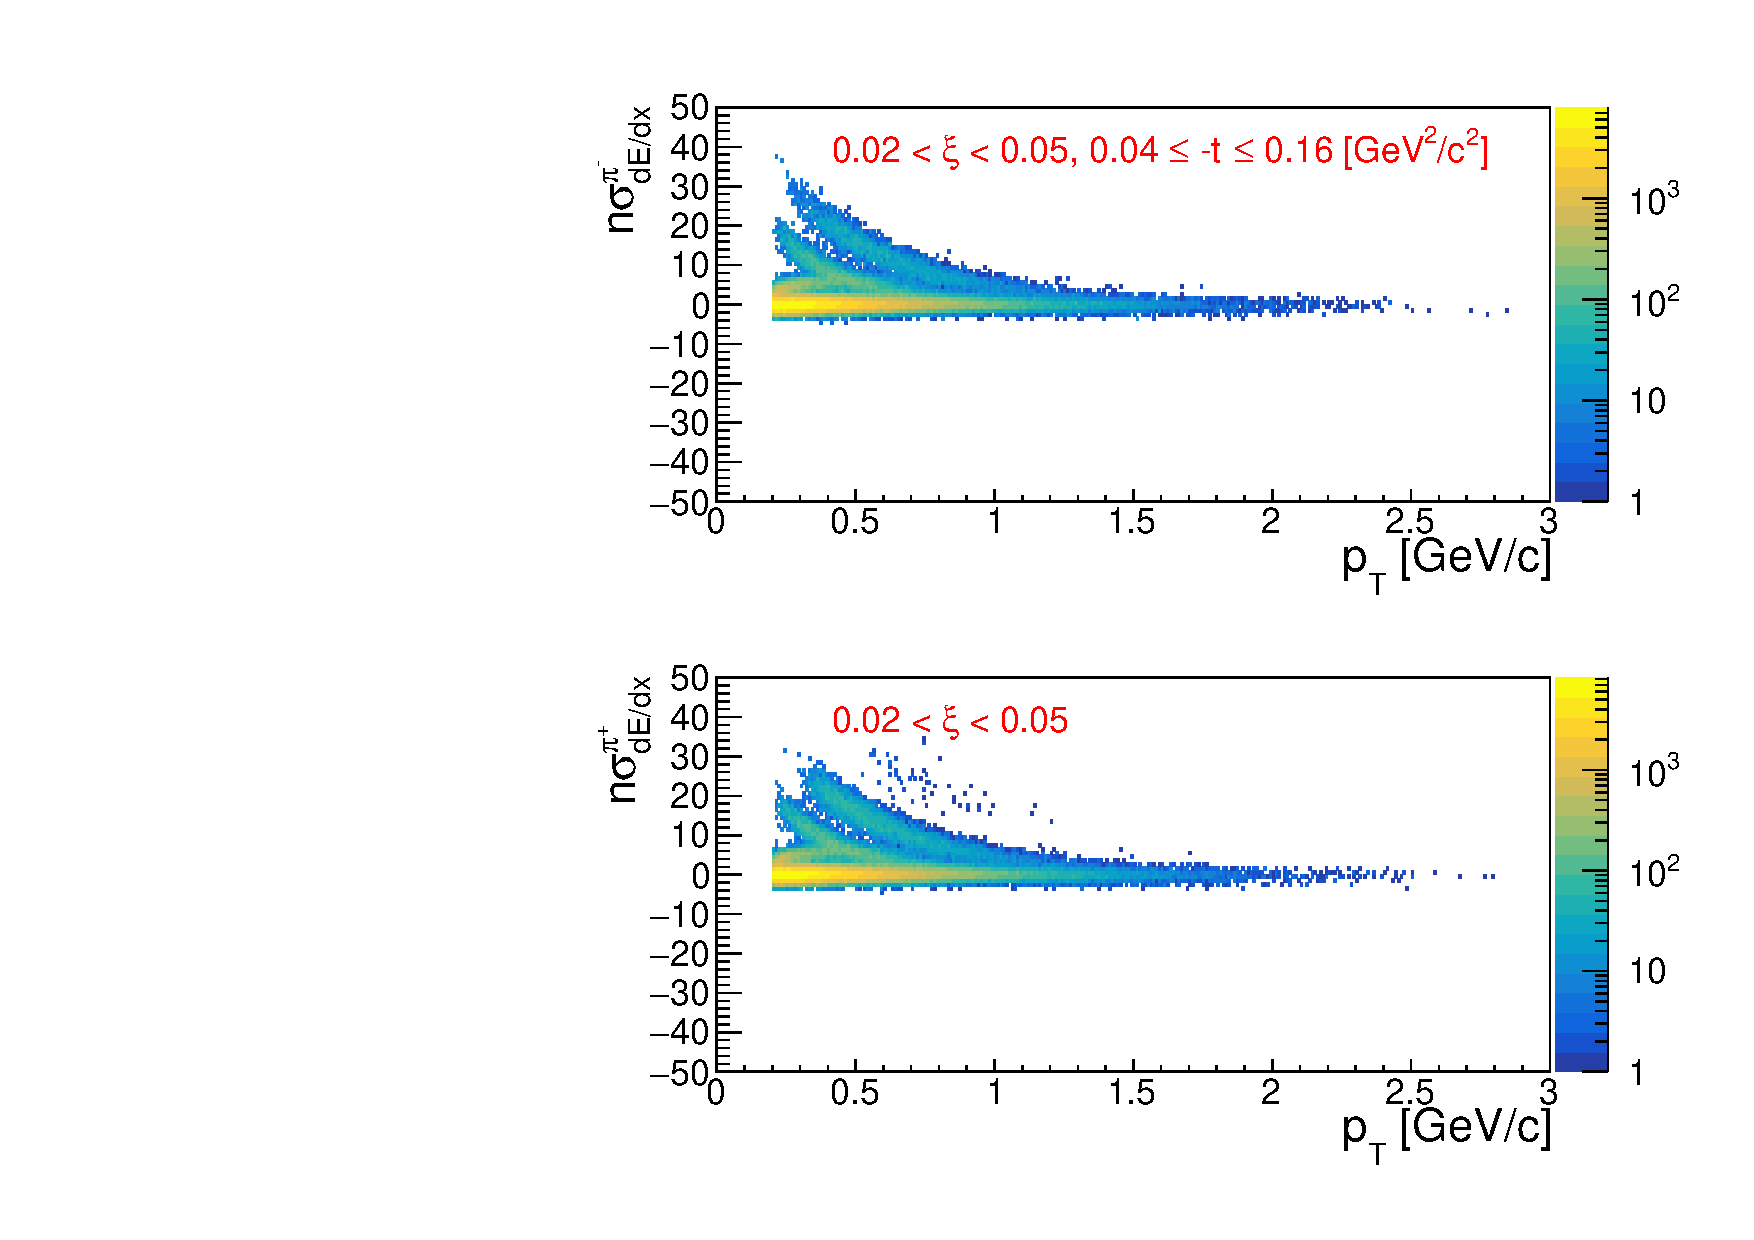
\includegraphics[width=\linewidth, page=1]{chapters/chrgSTAR/img/dEdx/fit2019_2dNsigma_0_0.pdf}
	\end{subfigure}
	\begin{subfigure}{.49\textwidth}
		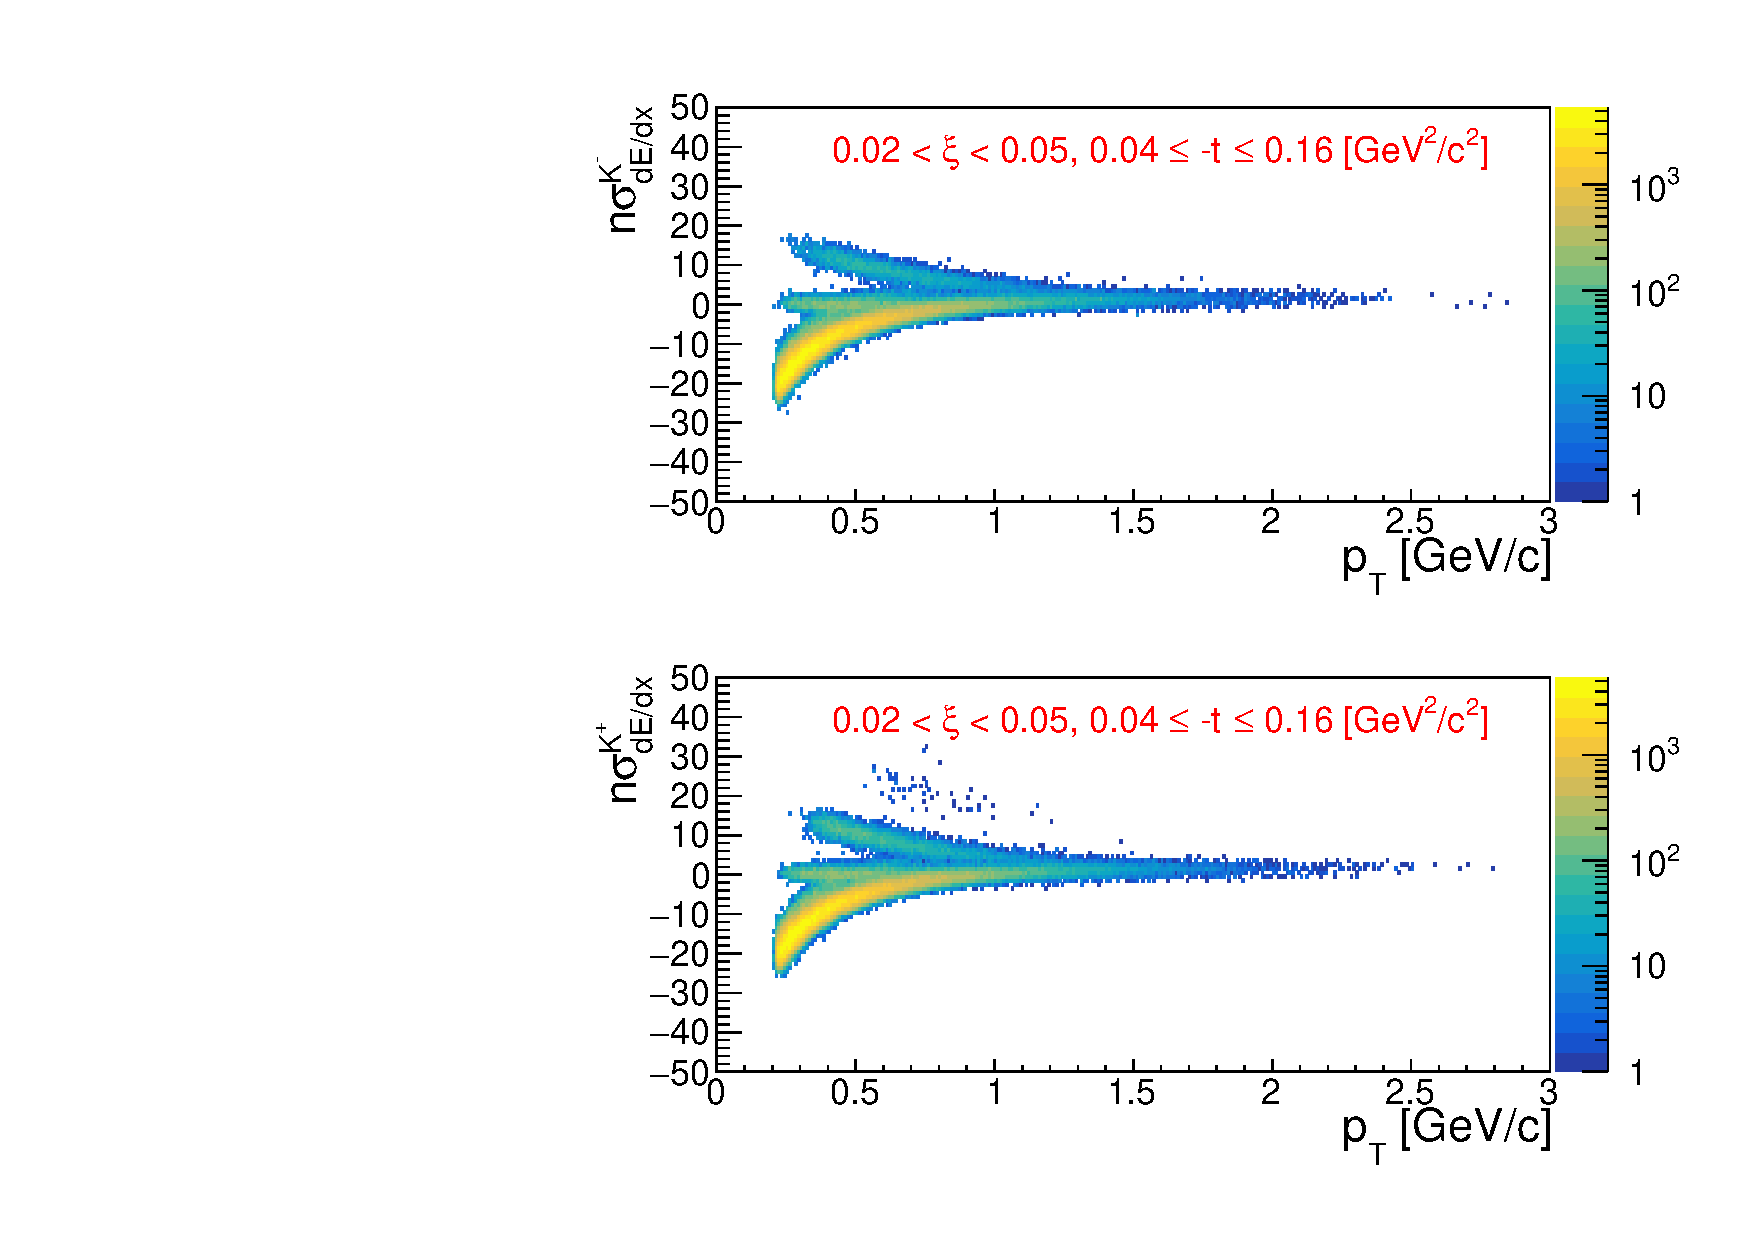
\includegraphics[width=\linewidth, page=1]{chapters/chrgSTAR/img/dEdx/fit2019_2dNsigma_0_1.pdf}
	\end{subfigure}
	\begin{subfigure}{.49\textwidth}
		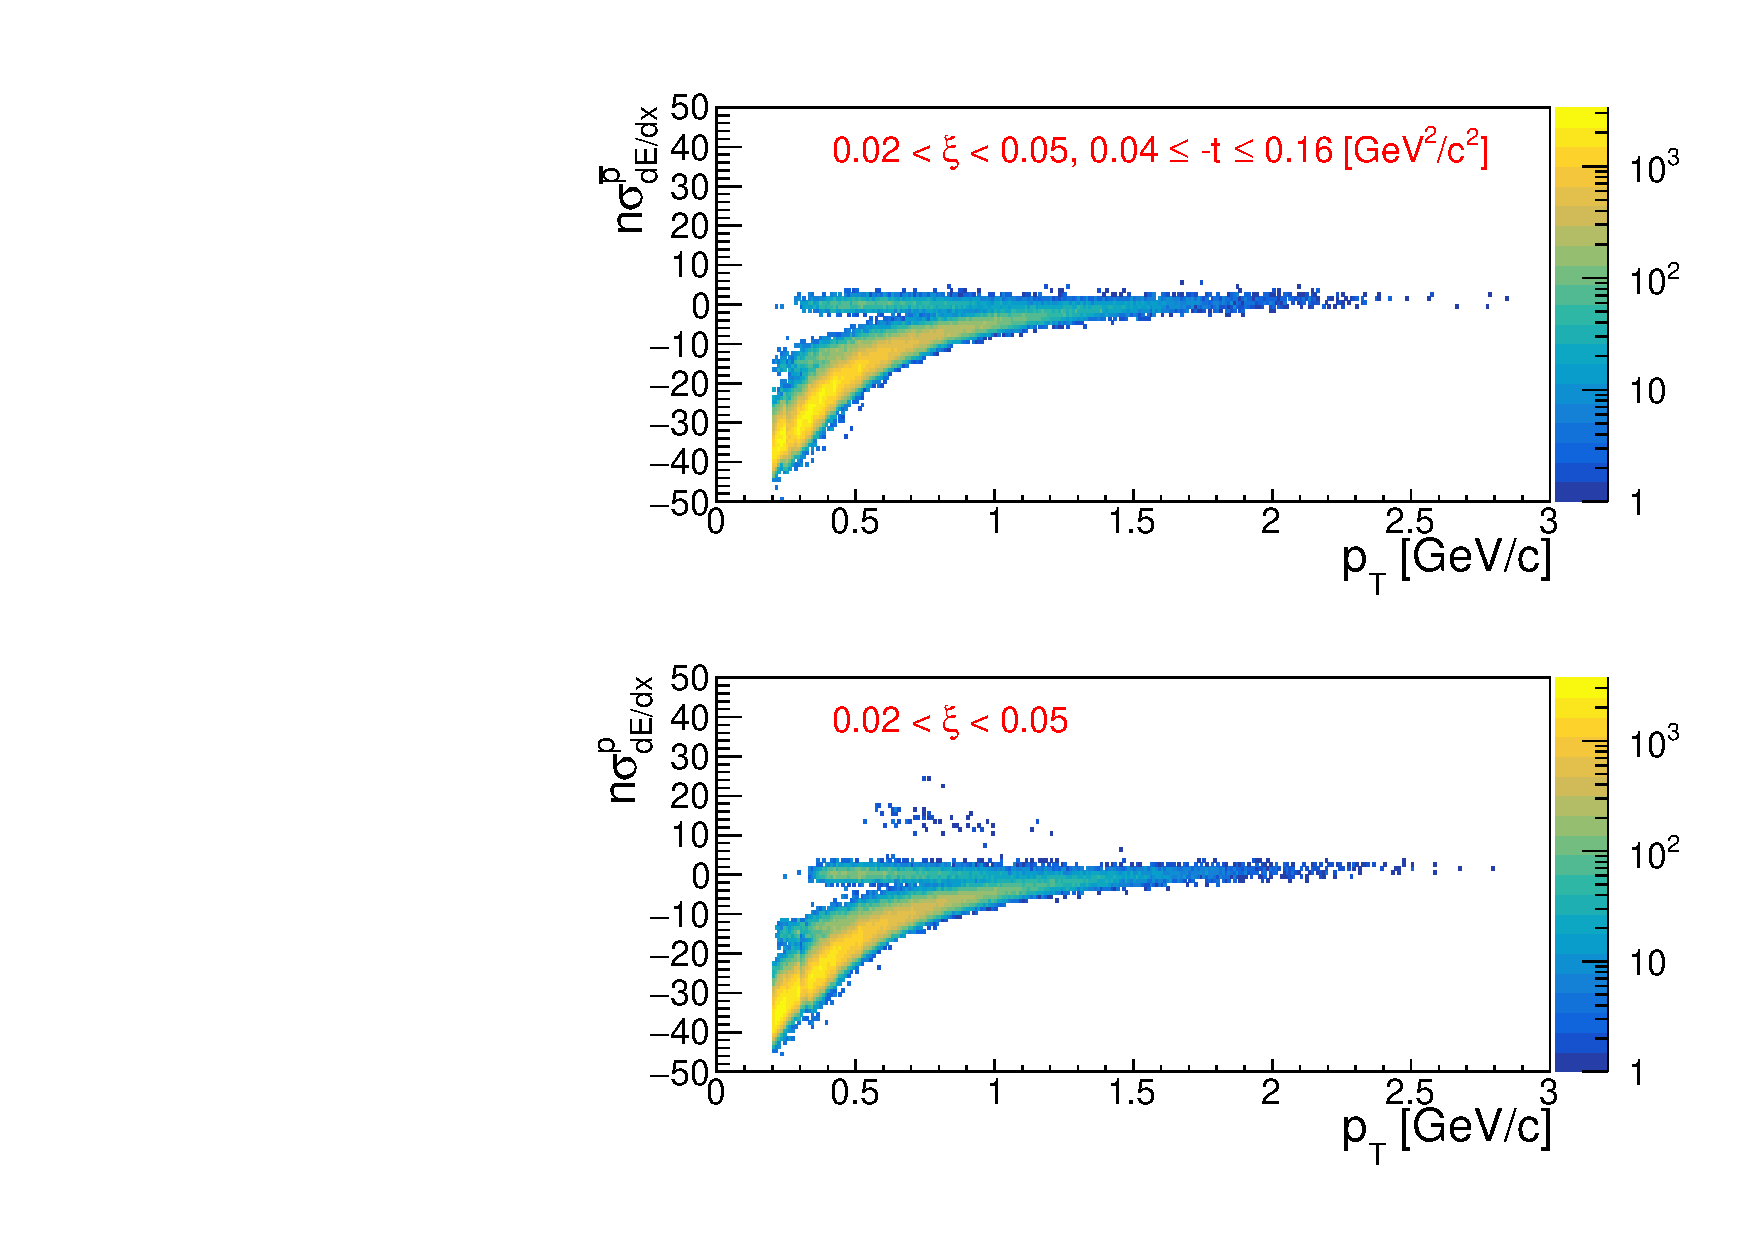
\includegraphics[width=\linewidth, page=1]{chapters/chrgSTAR/img/dEdx/fit2019_2dNsigma_0_2.pdf}
	\end{subfigure}
	\begin{minipage}{.49\textwidth}
			\caption{
			The $n\sigma^{i}_{dE/dx}$ variable for particle $i^\pm$ versus $p_\textrm{T}$. Particles are restricted in $|\eta| < 0.7$ and corrected for the energy loss (mass of $i^\pm$-particle was taken)~\cite{supplementaryNote} and vertexing.}
		\label{fig:dEdx_nsigma}
	\end{minipage}
	\vspace{1em}
\end{figure}

\begin{figure}[h!]
	\centering
	\begin{subfigure}{.49\textwidth}
		\includegraphics[width=\linewidth, page=9]{chapters/chrgSTAR/img/dEdx/fit2019_secondStep_0_0.pdf}
	\end{subfigure}
	\begin{subfigure}{.49\textwidth}
		\includegraphics[width=\linewidth, page=7]{chapters/chrgSTAR/img/dEdx/fit2019_thirdStep_1_0.pdf}
	\end{subfigure}\par
	\begin{subfigure}{.49\textwidth}
		\includegraphics[width=\linewidth, page=5]{chapters/chrgSTAR/img/dEdx/fit2019_thirdStep_2_0.pdf}
	\end{subfigure}
	\begin{minipage}{.49\textwidth}
		\caption{Distributions of (top left) $n\sigma^{\pi^\pm}_{dE/dx}$ for $\pi^\pm$, (top right) $n\sigma^{K^\pm}_{dE/dx}$ for $K^\pm$ and (bottom left) $n\sigma^{\bar{p}/p}_{dE/dx}$ for $\bar{p}/p$ in sample  $p_\textrm{T}$ bin and sample $\xi$ range  shown for each particle species. Particles are corrected for  energy loss~\cite{supplementaryNote} and vertexing. The curves represent the Gaussian fits to the $n\sigma^{i}_{dE/dx}$ distributions.}
		\label{fig:dEdx_fit_example}
	\end{minipage}
	
\end{figure}


\noindent Figure \ref{fig:dEdx_fit_example}
shows the $n\sigma^{\pi^\pm}_{dE/dx}$,$n\sigma^{K^\pm}_{dE/dx}$ and $n\sigma^{p(\bar{p})}_{dE/dx}$ distributions for  $0.6 < p_\textrm{T} < 0.65$~GeV/c  in the~$\xi$ range, $0.02 < \xi < 0.05$, each corrected for the energy loss (mass of $i$-particle was assumed)~\cite{supplementaryNote} and vertexing  (other $p_\textrm{T}$ bins are shown in Appendix~\ref{appendix:dEdxFits}). To extract the  particle yield for a given particle type,
a~multi-Gaussian fit is applied to the $n\sigma^i_{dE/dx}$ distribution in each $p_\textrm{T}$ bin and $\xi$ range. The parameters of the multi-Gaussian fit are the centroids $\mu_{i^-/i^+}$, widths $\sigma_{i^-/i^+}$, sums  and ratios  of yields $C_{i^-/i^+}$, $r_{i^-/i^+}$ for negative $i^-$ and positive $i^+$ particles ($\pi^\pm$, $e^\pm$, $K^\pm$, $p$ and $\bar{p}$). The~positive and negative particle
$n\sigma^{i}_{dE/dx}$-distributions are fitted simultaneously, where the~centroids and widths are kept the same for particle
and antiparticle. 
In some $p_\textrm{T}$ regions, the~fit does not converge,
because different particle species are not well separated  there. Therefore, multiple steps of the~fitting procedure  are performed to reduce the number of free parameters in the final fit and ensure its stability. Almost all centroids and widths are constrained  by a~function with free parameters $p_k$, where $k \in \mathbb N$.  The function is chosen to describe the data as best as possible.
Since $dE/dx$ is a~function of the~particle's momentum and its shape should be independent of the~process under study, the values of $p_k$  are obtained only for events with $0.02 < \xi < 0.05$ and kept the same for other $\xi$ ranges. The electron contributions are fitted only at $p_\textrm{T}<0.4$~GeV/c, separately for each
particle species and $\xi$ range. For higher $p_\text{T}$ ranges, they are estimated from PYTHIA 8 embedding MC, and scaled according to the ratio of PYTHIA 8 predictions and contributions
fitted in the $0.35<p_\textrm{T}<0.4$~GeV/c  bin.
The procedure slightly differs for different particle types. In each step, the~multi-Gaussian fit is performed first, then the~widths and centroids are fitted  in  $p_\textrm{T}$ ranges in which the fit applied to $n\sigma^{i}_{dE/dx}$ converges. Later,  the~widths and centroids are extrapolated to other $p_\textrm{T}$ ranges, in which particle species are not well separated:
%\newpage
\begin{enumerate}
	\item  $\pi^{\pm}$:
		\begin{itemize}
			\item Step 1 (Fig. ~\ref{fig:dEdx_fit_parametersPi}):
			\begin{itemize}
				\renewcommand\labelitemi{--}
				\item Analyze data with $0.2 < p_\textrm{T} < 0.65$~GeV/c
				\item Fit  $\mu_{\pi^-/\pi^+}$ and $\sigma_{\pi^-/\pi^+}$ as a function of $p_\textrm{T}$ with a polynomial  $p_0p_\textrm{T}^3+p_1p_\textrm{T}^2+p_2p_\textrm{T}+p_3$
				%\item Fit $r_{e^-/e^+}$ as a function of $p_\textrm{T}$ with a polynomial $p_0p_\textrm{T}^2+p_1p_\textrm{T}+p_2$
				\item Fit  %$C_{e^-/e^+}$, 
				$\mu_{K^-/K^+}$ as a function of $p_\textrm{T}$ with $p_0\exp\left(p_1p_\textrm{T}\right)+p_2$
				\item Fit  $\mu_{e^-/e^+}$ as a function of $p_\textrm{T}$ with $p_0\exp\left[-\left(p_1p_\textrm{T}\right)^{p_2}\right]$ 
				\item Fit $\sigma_{K^-/K^+}$ as a function of $p_\textrm{T}$, for $0.3<p_\textrm{T}<0.5$~GeV/c, with constant $p_0$ 
				\item Fit  $\mu_{\bar{p}/p}$ and $\sigma_{\bar{p}/p}$ as a function of $p_\textrm{T}$ with $p_0\exp\left(p_1p_\textrm{T}\right)$
			\end{itemize}
			\item Step 2:
				\begin{itemize}
					\renewcommand\labelitemi{--}
					\item $\sigma_{e^-/e^+}$ fixed to $1.2$ and $0.8$ for $0.2<p_\textrm{T}<0.4$ and $0.4<p_\textrm{T}<0.7$, respectively
					\item Fit $\sigma_{K^-/K^+}$ as a function of $p_\textrm{T}$, for $0.3<p_\textrm{T}<0.7$~GeV/c, with constant $p_0$ and fix it to the~value of $p_0$
					\item  The rest parameters from Step 1 are fixed to the~values calculated from functions obtained in Step 1: $\mu_{\pi^-/\pi^+}$, $\sigma_{\pi^-/\pi^+}$,  % $r_{e^-/e^+}$, $C_{e^-/e^+}$, 
					$\mu_{e^-/e^+}$ , $\mu_{K^-/K^+}$, $\mu_{\bar{p}/p}$, $\sigma_{\bar{p}/p}$
				\end{itemize}	
		\end{itemize}		
\end{enumerate} 

\begin{enumerate}
	\item[2.] $K^\pm$:
	\begin{itemize}
		\item Step 1 (Fig. ~\ref{fig:dEdx_fit_parametersK}):
		\begin{itemize}
			\renewcommand\labelitemi{--}
			\item Analyze data with $0.2 < p_\textrm{T} < 0.6$~GeV/c
			\item Fit  $\mu_{\pi^-/\pi^+}$  as a function of $p_\textrm{T}$ with $-\exp\left(p_0+p_1p_\textrm{T}\right)$
			\item Fit $\sigma_{\pi^-/\pi^+}$, %$C_{e^-/e^+}$, 
			$\sigma_{e^-/e^+}$, $\sigma_{K^-/K^+}$ as a function of $p_\textrm{T}$ with $\exp\left(p_0+p_1p_\textrm{T}\right)$
			%\item Fit $r_{e^-/e^+}$ as a function of $p_\textrm{T}$ with constant $p_0$ 
			\item Fit $\mu_{e^-/e^+}$ as a function of $p_\textrm{T}$ with a~polynomial  $p_0p_\textrm{T}^3+p_1p_\textrm{T}^2+p_2p_\textrm{T}+p_3$
			\item Fit $\mu_{K^-/K^+}$ as a function of $p_\textrm{T}$ with a~polynomial  $p_0+p_1p_\textrm{T}^2$
			
		\end{itemize}
		\item Step 2:
		\begin{itemize}
			\renewcommand\labelitemi{--}
			\item All parameters from Step 1 except $\sigma_{e^-/e^+}$ are fixed to the~values calculated from functions obtained in Step 1
			\item  Fit $\sigma_{e^-/e^+}$ as a function of $p_\textrm{T}$, for $0.45<p_\textrm{T}<0.65$~GeV/c, with constant $p_0$ 
			
		\end{itemize}
		\item Step 3:
		\begin{itemize}
			\renewcommand\labelitemi{--}
			\item  $\sigma_{e^-/e^+}$ fixed to the~values calculated from functions obtained in  Steps 1 and 2 for $0.3<p_\textrm{T}<0.45$ and $0.45<p_\textrm{T}<0.65$, respectively.
			\item  The rest parameters from Step 1 are fixed to the~values calculated from functions obtained in Step 1: $\mu_{\pi^-/\pi^+}$, $\sigma_{\pi^-/\pi^+}$, %$r_{e^-/e^+}$, $C_{e^-/e^+}$, 
			$\mu_{e^-/e^+}$ , $\mu_{K^-/K^+}$,$\sigma_{K^-/K^+}$
		\end{itemize}		
	\end{itemize}		
\end{enumerate} 

\begin{figure}[h!]
	\centering
	\begin{subfigure}{.32\textwidth}
		\includegraphics[width=\linewidth, page=3]{chapters/chrgSTAR/img/dEdx/fit2019_fitResult_0_0_step_0.pdf}
	\end{subfigure}
	\begin{subfigure}{.32\textwidth}
		\includegraphics[width=\linewidth, page=4]{chapters/chrgSTAR/img/dEdx/fit2019_fitResult_0_0_step_0.pdf}
	\end{subfigure}
	\begin{subfigure}{.32\textwidth}
		\includegraphics[width=\linewidth, page=5]{chapters/chrgSTAR/img/dEdx/fit2019_fitResult_0_0_step_0.pdf}
	\end{subfigure}
	\begin{subfigure}{.32\textwidth}
		\includegraphics[width=\linewidth, page=6]{chapters/chrgSTAR/img/dEdx/fit2019_fitResult_0_0_step_0.pdf}
	\end{subfigure}
	\begin{subfigure}{.32\textwidth}
		\includegraphics[width=\linewidth, page=7]{chapters/chrgSTAR/img/dEdx/fit2019_fitResult_0_0_step_0.pdf}
	\end{subfigure}
	\begin{subfigure}{.32\textwidth}
		\includegraphics[width=\linewidth, page=8]{chapters/chrgSTAR/img/dEdx/fit2019_fitResult_0_0_step_0.pdf}
	\end{subfigure}
	\begin{subfigure}{.32\textwidth}
		\includegraphics[width=\linewidth, page=11]{chapters/chrgSTAR/img/dEdx/fit2019_fitResult_0_0_step_0.pdf}
	\end{subfigure}
	\begin{subfigure}{.32\textwidth}
		\includegraphics[width=\linewidth, page=12]{chapters/chrgSTAR/img/dEdx/fit2019_fitResult_0_0_step_0.pdf}
	\end{subfigure}
	\begin{subfigure}{.32\textwidth}
		\includegraphics[width=\linewidth, page=15]{chapters/chrgSTAR/img/dEdx/fit2019_fitResult_0_0_step_0.pdf}
	\end{subfigure}
	\begin{subfigure}{.32\textwidth}
		\includegraphics[width=\linewidth, page=16]{chapters/chrgSTAR/img/dEdx/fit2019_fitResult_0_0_step_0.pdf}
	\end{subfigure}
	\begin{minipage}{.64\textwidth}
		\caption{Means, widths and electron yields of each $n\sigma^{\pi^\pm}_{dE/dx}$ fit as a function of $p_\textrm{T}$.  The red line on each plot is a~fit function to stabilize and constrain the Gaussian fit parameters for the final fitting step.}
		\label{fig:dEdx_fit_parametersPi}
	\end{minipage}
	
\end{figure}
\begin{enumerate}
	\item[3.] $\bar{p},p$:
	\begin{itemize}
		\item Step 1 (Fig. ~\ref{fig:dEdx_fit_parameters_P}):
		\begin{itemize}
			\renewcommand\labelitemi{--}
			\item Analyze data with $0.4 < p_\textrm{T} < 0.9$~GeV/c
			\item Fit  $\mu_{\pi^-/\pi^+}$, $\mu_{K^-/K^+}$   as a function of $p_\textrm{T}$ with a~polynomial  $p_0p_\textrm{T}+p_1$ 
			\item Fit  $\sigma_{\pi^-/\pi^+}$  as a function of $p_\textrm{T}$ with a~polynomial $p_0p_\textrm{T}^2+p_1p_\textrm{T}+p_2$ 
			\item Fit $\sigma_{K^-/K^+}$ as a function of $p_\textrm{T}$ with $\exp\left(p_0+p_1p_\textrm{T}\right)$
		\end{itemize}
		\item Step 2:
		\begin{itemize}
			\renewcommand\labelitemi{--}
			\item $\mu_{K^-/K^+}$ fixed to the~values calculated from a~function obtained in Step 1
			\item All the rest parameters from Step 1 are limited to the~values calculated from functions obtained in Step 1
			\item Fit  $\mu_{\pi^-/\pi^+}$, $\sigma_{\pi^-/\pi^+}$, $\sigma_{K^-/K^+}$  as a function of $p_\textrm{T}$ with a~polynomial $p_0p_\textrm{T}^2+p_1p_\textrm{T}+p_2$ 
			\item Fit  $\mu_{\bar{p}/p}$  as a function of $p_\textrm{T}$, for $0.7<p_\textrm{T}<1.0$~GeV/c, with constant $p_0$ 
			
		\end{itemize}
		\item Step 3:
		\begin{itemize}
			\renewcommand\labelitemi{--}
			\item  $\mu_{K^-/K^+}$ fixed to the~values calculated from a~function obtained in Step 1
			\item $\mu_{\bar{p}/p}$  fixed to the~values calculated from a~function obtained in Step 2 for $0.7<p_\textrm{T}<1.0$
			\item  The rest parameters from Step 2 are fixed to the~values calculated from functions obtained in Step 2: $\mu_{\pi^-/\pi^+}$, $\sigma_{\pi^-/\pi^+}$, $\sigma_{K^-/K^+}$
		\end{itemize}		
	\end{itemize}		
\end{enumerate} 
\begin{figure}[h!]
	\centering
	\begin{subfigure}{.32\textwidth}
		\includegraphics[width=\linewidth, page=3]{chapters/chrgSTAR/img/dEdx/fit2019_fitResult_1_0_step_0.pdf}
	\end{subfigure}
	\begin{subfigure}{.32\textwidth}
		\includegraphics[width=\linewidth, page=4]{chapters/chrgSTAR/img/dEdx/fit2019_fitResult_1_0_step_0.pdf}
	\end{subfigure}
	\begin{subfigure}{.32\textwidth}
		\includegraphics[width=\linewidth, page=5]{chapters/chrgSTAR/img/dEdx/fit2019_fitResult_1_0_step_0.pdf}
	\end{subfigure}
	\begin{subfigure}{.32\textwidth}
		\includegraphics[width=\linewidth, page=6]{chapters/chrgSTAR/img/dEdx/fit2019_fitResult_1_0_step_0.pdf}
	\end{subfigure}
	\begin{subfigure}{.32\textwidth}
		\includegraphics[width=\linewidth, page=7]{chapters/chrgSTAR/img/dEdx/fit2019_fitResult_1_0_step_0.pdf}
	\end{subfigure}
	\begin{subfigure}{.32\textwidth}
		\includegraphics[width=\linewidth, page=8]{chapters/chrgSTAR/img/dEdx/fit2019_fitResult_1_0_step_0.pdf}
	\end{subfigure}
	\begin{subfigure}{.32\textwidth}
		\includegraphics[width=\linewidth, page=11]{chapters/chrgSTAR/img/dEdx/fit2019_fitResult_1_0_step_0.pdf}
	\end{subfigure}
	\begin{subfigure}{.32\textwidth}
		\includegraphics[width=\linewidth, page=12]{chapters/chrgSTAR/img/dEdx/fit2019_fitResult_1_0_step_0.pdf}
	\end{subfigure}
	\caption{Means, widths and electron yields of each $n\sigma^{K^\pm}_{dE/dx}$ fit as a function of $p_\textrm{T}$.  The red line on each plot is a~fit function to stabilize and constrain the Gaussian fit parameters for the final fitting step.}
	\label{fig:dEdx_fit_parametersK}
	%\vspace{-2cm}
\end{figure}

\begin{figure}[h!]
	\centering
	\begin{subfigure}{.32\textwidth}
		\includegraphics[width=\linewidth, page=3]{chapters/chrgSTAR/img/dEdx/fit2019_fitResult_2_0_step_1.pdf}
	\end{subfigure}
	\begin{subfigure}{.32\textwidth}
		\includegraphics[width=\linewidth, page=4]{chapters/chrgSTAR/img/dEdx/fit2019_fitResult_2_0_step_1.pdf}
	\end{subfigure}
	\begin{subfigure}{.32\textwidth}
		\includegraphics[width=\linewidth, page=11]{chapters/chrgSTAR/img/dEdx/fit2019_fitResult_2_0_step_0.pdf}%done
	\end{subfigure}
	\begin{subfigure}{.32\textwidth}
		\includegraphics[width=\linewidth, page=12]{chapters/chrgSTAR/img/dEdx/fit2019_fitResult_2_0_step_1.pdf}
	\end{subfigure}
		\begin{subfigure}{.32\textwidth}
			\includegraphics[width=\linewidth, page=15]{chapters/chrgSTAR/img/dEdx/fit2019_fitResult_2_0_step_1.pdf}
		\end{subfigure}
	\caption{Means and widths  of each $n\sigma^{\bar{p}/p}_{dE/dx}$ fit as a function of $p_\textrm{T}$.  The red line on each plot is a~fit function to stabilize and constrain the Gaussian fit parameters for the final fitting step.}
	\label{fig:dEdx_fit_parameters_P}
	
\end{figure}


The particle yield is extracted from the fit to the corresponding
$n\sigma^{i}_{dE/dx}$  distribution (corrected only for the energy loss and vertexing). As shown in Fig.~\ref{fig:dEdx_nsigma}, the $dE/dx$ of each particle type merge at large $p_\textrm{T}$. Hence, the particle identification is limited. Pions can be identified
in the momentum range of $0.2-0.7$~GeV/c, kaons in
$0.3-0.65$~GeV/c and (anti)protons in $0.4-1.0$~GeV/c. 
\FloatBarrier

%ratios
\subsection{Antiparticle-to-Particle Ratios}\label{section:star_ratios}
The following steps were taken to correct an  identified antiparticle to particle (pion, kaon, proton and their antiparticle) multiplicity ratios as a function of $p_T$ in three ranges of $\xi$.
\begin{itemize}
	\item The raw identified particle yields were obtained through multi-Gaussian fits to the $n\sigma^i_{dE/dx}$ distributions (Sec.~\ref{section:star_PIDdEdx}), where the vertex reconstruction and energy loss corrections were applied. The latter depends on the particle type.
	\item The accidental and non-SD backgrounds were subtracted. It was assumed that the former does not depend on the particle type, i.e. the same contribution of accidental background was used as for charged particles without identification (Sec.~\ref{section:star_accidentals}).
	\item The particle yields were corrected for track reconstruction efficiencies, which depend on the particle type and charge.
	\item The background from non-primary tracks was subtracted (Sec.~\ref{section:star_background_primary}):
	\begin{itemize}
		\item $\pi^\pm$: weak decays pions, muon contribution and background from  detector dead-material interactions,
		\item $p$: background from  detector dead-material interactions,
		\item $p,\bar{p}$: reconstructed tracks which have the appropriate number of common hit points with true-level particle, but the distance between them is too large (this background is negligibly small for other particle types),
		\item all: fake track contribution, the same for each particle type. 
	\end{itemize}
	\item Then the tracks were corrected for track and $\xi$ migrations, BBC-small efficiency, which do not depend on the particle type and charge.
	\item Finally, each antiparticle $p_T$ distribution was divided by the corresponding particle $p_T$ distribution to obtain fully corrected identified antiparticle to particle multiplicity ratios.
	\item Additionally, the average antiparticle to particle ratios in each $\xi$ region were calculated.
\end{itemize}
